% LaTeX Datei für Projektberichte
\documentclass[12pt,a4paper,oneside]{article}

%---------------------------------------------------------------
%	Pakete
%---------------------------------------------------------------

%\usepackage{tikz}
%\usepackage[ngerman]{babel}            %   neue deutsche Rechtschreibung
%\usepackage[utf8]{inputenc}
%\usepackage[T1]{fontenc}
%\usepackage{subfigure} 
%\usepackage{multirow}
%\usepackage[table,xcdraw]{xcolor}

%\usepackage{color}
%\usepackage{graphicx}
%\usepackage[table,xcdraw]{xcolor}
%\usepackage{setspace}
%\usepackage[title,titletoc,toc]{appendix}
%\usepackage{geometry}
%\geometry{a4paper,left=19mm,right=19mm, top=25mm, bottom=25mm}
%\usetikzlibrary{shapes.geometric, arrows}

\usepackage[utf8]{inputenc}
\usepackage[T1]{fontenc}
\usepackage{multirow}
\usepackage[table,xcdraw]{xcolor}

\usepackage{color}
\usepackage{graphicx}
\usepackage[table,xcdraw]{xcolor}
\usepackage{setspace}
\usepackage[title,titletoc,toc]{appendix}
\usepackage{geometry}
\geometry{a4paper,left=19mm,right=19mm, top=25mm, bottom=25mm}








\usepackage{tikz}
\usepackage[ngerman]{babel}            %   neue deutsche Rechtschreibung
\usepackage[utf8]{inputenc}
\usepackage[T1]{fontenc}
\usepackage{color}
\usepackage{graphicx}
\usepackage{subfigure}
\usepackage[table,xcdraw]{xcolor}
\usepackage{setspace}
\usepackage{setspace}
\usepackage[title,titletoc,toc]{appendix}
\usepackage{geometry}
\geometry{a4paper,left=19mm,right=19mm, top=25mm, bottom=25mm}
\usetikzlibrary{shapes.geometric, arrows}


%---------------------------------------------------------------
% Dokumentenanfang:
%---------------------------------------------------------------
\begin{document}                            % Dokumentenanfang
	\usetikzlibrary{shapes,arrows}
\begin{spacing}{1.15}                       % Zeilenabstand 1,15

	\begin{titlepage}

\begin{flushleft}
	
\includegraphics[height=1.5cm]{figs/LKR_Logo.png}
	\hfill
	%\includegraphics[height=1.5cm]{figs/MZH_Logo.png}
	%\hfill
	
\includegraphics[height=1.5cm]{figs/LUH_Logo.jpg}
\end{flushleft}

\vspace{10mm} 
\begin{center}
\Large{Vorlesung/Experimentelle \"Ubung: 

Programmierung mechatronischer Systeme

\vspace{5mm}

\textbf{Hausarbeit}}

\vspace{5mm}
\textbf{\LARGE{Raspberry Pi Roboter ("French Bulldog")}}
\end{center}

\vfill
% hier könnt ihr ein Bild eurer Roboters einfügen
\begin{center}
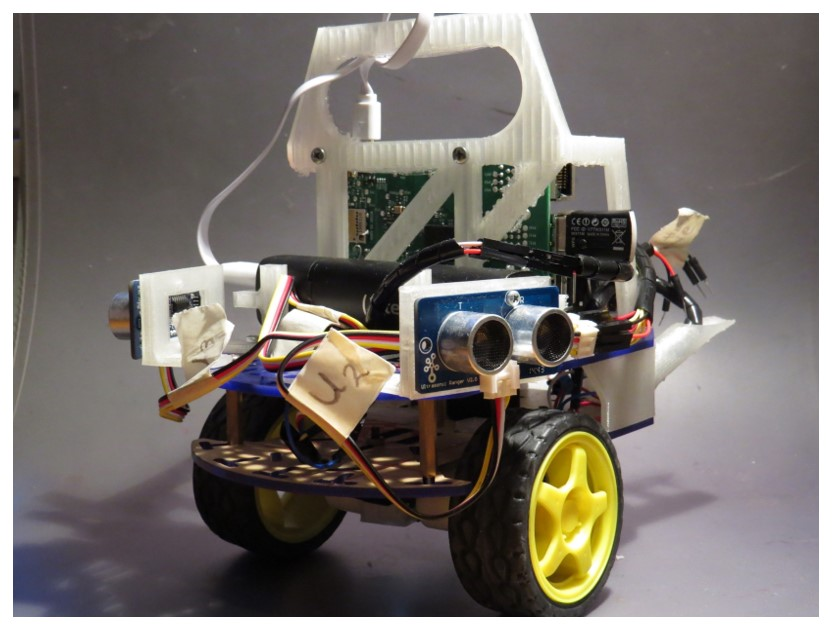
\includegraphics[width = 80mm]{figs/PiRobot.jpg}
\end{center}

\vfill

\begin{center}
\begin{tabular}{c c}
\large{Tobias Gieseking} & \large{Nils Melchert}\\
\large{Matrikelnummer 2883510} & \large{Matrikelnummer 2869520}
\end{tabular}
\end{center}
\vspace{15mm}

\begin{tabular}{l}
\large{Sommersemester 2016}\\
\large{Hannover, 15.07.2016}
\end{tabular}


\vspace{15mm}
{\large
\begin{tabular}{l l}
Dozentin:  & Prof. Dr.-Ing. Jessica Burgner\\
Betreuer: & M.Sc. Ernar Amanov und M.Sc. Carolin Fellmann\\
\end{tabular}
}

\end{titlepage}

    \clearpage
    \tableofcontents                        % Inhaltsverzeichnis 
    \thispagestyle{empty}
    \clearpage   
	\setcounter{page}{1}
	%-----------------------------
	% Einleitung
	%-----------------------------	
	\section{Einleitung}
	
	Die vorliegende Hausarbeit dokumentiert das Gruppenergebnis des Team 2 namens \glqq French Bulldog\grqq\  aus dem Sommersemester 2016, welches während der Teilnahme an dem Kurs \glqq Programmierung mechatronischer Systeme\grqq\ (PMS) des Lehrstuhls für Kontinuumrobotik (LKR) unter der Leitung von Frau Prof. Jessica Burgner-Kahrs erarbeitet wurde.
	\vspace{2mm}\\
	Das Lehrziel der Veranstaltung war es die Grundlagen des objektorientierten Programmierens in C++, den Umgang mit Nebenläufigkeiten und den für C++ charakteristischen Pointern zu vermitteln. Außerdem sollten die Studenten einen sauberen Programmierstil zur Beherrschung  komplexer Programmierprojekte erlernen. Zur praktischen Untermauerung der Veranstaltung sollte ein einfacher Roboter, bestehend aus einem Einplatinencomputer und zwei Motoren sowie diverser Sensoren programmiert werden, der unterschiedliche Teilaufgaben zu bewältigen hatte. Den Studenten wurde die Möglichkeit gegeben das Zusammenspiel der vier Komponenten \glqq mechanisches System\grqq , \glqq Sensorik\grqq , \glqq Informatik\grqq\  und \glqq Aktorik\grqq\  eines mechatronischen Systems mit ihren Herausforderungen in der Praxis zu meistern. Parallel zur sauberen Programmierung war eine übersichtliche Kabelführung anzustreben, um vorallem in den vier über die Vorlesungszeit verteilten Prüfungssituationen Fehlfunktionen gezielt zurückverfolgen zu können. Weitere Schwerpunkte der Vorlesung waren die Nutzung der IDE Qt-Creator, das Auslegen von Reglern für die Drehzahlsteuerung der Motoren und das Implementieren eines $I^{2}C$-Buses zur Nutzung eines Farbsensors.
	
	Die Hausarbeit beginnt mit der Vorstellung des Roboters hardwareseitig. Es werden die einzelnen Komponenten beschrieben, warum die Komponenten ausgewählt wurden und aus welchen Gründen spezifische Positionierungen am Roboter ausgewählt wurden. Im zweiten Teil werden die Programmieransätze zu den vier Meilensteinen erläutert. Unterstützend finden sich an dieser Stelle Klassendiagramme und Programmablaufpläne. Im anschließenden Teil werden aufgetretene Probleme und Herausforderungen diskutiert. Standardmäßig schließt das Dokument mit der Zusammenfassung des Erlernten und mit einem Ausblick.   
	
%-----------------------------
% Der Roboter
%-----------------------------
\section{Der Roboter}

In diesem Kapitel wird der Hardware des Roboters erläutert. Zunächst wird in 2.1 ein Überblick über die verwendeten Komponenten gegeben. Es wird mit kurzer Beründung gezeigt, wo sie warum Montiert wurden. Dabei soll etwas detaillierter auf das Gehirn des Roboters, den Raspberry Pi, eingegangen werden. Dieser Teil war bei den meisten Team ähnlich, da alle das selbe Chassi verwendeten und z.B. die Motoren nur an einer definierten Stelle platziert werden konnten. Unterscheiden tun sich die Roboter in der Auswahl der Sensoren, darum wird in 2.2 auf diese detailert eingegangen. 

\subsection{Mobile Plattform}

Das Grundgerüst der mobilen Roboterplattform bildete das \textit{Dagu Magician Chassis}, welches aus zwei Platikplatten mit einer Vielzahl von Bohrungen und Nuten bestand. Es bildete die formgebende Komponente des Roboters und besitzt  die Maße $11 17,5 7,5$ in Zentimetern. 

\begin{table}[h]
	\centering
	\caption{My caption}
	\label{my-label}
	\begin{tabular}{lll}
		\hline
		\rowcolor[HTML]{9B9B9B} 
		\multicolumn{1}{|l|}{\cellcolor[HTML]{9B9B9B}\textbf{Komponente}} & \multicolumn{1}{l|}{\cellcolor[HTML]{9B9B9B}\textbf{Abkürzung}} & \multicolumn{1}{l|}{\cellcolor[HTML]{9B9B9B}\textbf{Anzahl}} \\  \hline
		Raspberry Pi                                                      & 1\_Pi                                                           & 1                                                                                                                                                                                \\
		Motor                                                             & 2\_Mo                                                           & 2                                                                                                                                             \\
		Resolver                                                          & 3\_Rs                                                           & 2                                                                                                                                              \\
		H-Brücke                                                          & 4\_HB                                                           & 1                                                                                                                                                   \\
		Ultraschallsensor                                                 & 5\_Us                                                           & 2                                                                                                                                        \\
		Farbsensor                                                        & 6\_Fs                                                           & 1                                                                                                                                            \\
		Breadboard                                                        & 7\_Bb                                                           & 1                                                                                                                         \\
		Blockbatterie 9V                                                  & 8\_B9                                                           & 1                                                                                                                                         \\
		Powerbank 5V                                                      & 10\_Pb                                                          & 1                                                                                                                                        \\
		Jumperkabel                                                       & 11\_Jk                                                          & k.A.                                                                                                                          \\
		Widerstände                                                       & 12\_Ws                                                          & k.A.                                                                                                             
	\end{tabular}
\end{table}






\begin{table}[h]
	\centering
	\caption{Pinbelegungstabelle der GPIO-Pins des Raspberry Pis}
	\label{my-label}
	\begin{tabular}{lllll}
		\hline
		\rowcolor[HTML]{9B9B9B} 
		\multicolumn{1}{|l|}{\cellcolor[HTML]{9B9B9B}\textbf{\begin{tabular}[c]{@{}l@{}}wiringPi Bibl.\\ Pin Nr.\end{tabular}}} & \multicolumn{1}{l|}{\cellcolor[HTML]{9B9B9B}\textbf{\begin{tabular}[c]{@{}l@{}}Raspb. Pi \\ Pin Nr.\end{tabular}}} & \multicolumn{1}{l|}{\cellcolor[HTML]{9B9B9B}\textbf{}} & \multicolumn{1}{l|}{\cellcolor[HTML]{9B9B9B}\textbf{\begin{tabular}[c]{@{}l@{}}Verbunden \\ mit Pin\end{tabular}}} & \multicolumn{1}{l|}{\cellcolor[HTML]{9B9B9B}\textbf{Komponente}}                                           \\ \hline
		4                                                                                                                       & 16                                                                                                                 &                                                        & Hallsensor 1                                                                                                       &                                                                                                            \\
		5                                                                                                                       & 18                                                                                                                 &                                                        & Hallsensor 2                                                                                                       & \multirow{-2}{*}{\begin{tabular}[c]{@{}l@{}}Resolver rechter\\ Motor\end{tabular}}                         \\
		\rowcolor[HTML]{C0C0C0} 
		8                                                                                                                       & 3                                                                                                                  &                                                        & SLC                                                                                                                & \cellcolor[HTML]{C0C0C0}                                                                                   \\
		\rowcolor[HTML]{C0C0C0} 
		9                                                                                                                       & 5                                                                                                                  &                                                        & SDA                                                                                                                & \multirow{-2}{*}{\cellcolor[HTML]{C0C0C0}Farbsensor}                                                       \\
		12                                                                                                                      & 19                                                                                                                 &                                                        & SIG                                                                                                                & Ultraschallsensor 1                                                                                        \\
		13                                                                                                                      & 21                                                                                                                 &                                                        & SIG                                                                                                                & Ultraschallsensor 2                                                                                        \\
		\rowcolor[HTML]{C0C0C0} 
		15                                                                                                                      & 8                                                                                                                  &                                                        & Hallsensor 1                                                                                                       & \cellcolor[HTML]{C0C0C0}                                                                                   \\
		\rowcolor[HTML]{C0C0C0} 
		16                                                                                                                      & 10                                                                                                                 &                                                        & Hallsensor 2                                                                                                       & \multirow{-2}{*}{\cellcolor[HTML]{C0C0C0}\begin{tabular}[c]{@{}l@{}}Resolver linker \\ Motor\end{tabular}} \\
		23                                                                                                                      & 33                                                                                                                 &                                                        & 2                                                                                                                  &                                                                                                            \\
		24                                                                                                                      & 35                                                                                                                 &                                                        & 1                                                                                                                  &                                                                                                            \\
		25                                                                                                                      & 37                                                                                                                 &                                                        & 7                                                                                                                  & \multirow{-3}{*}{Motor links}                                                                              \\
		\rowcolor[HTML]{C0C0C0} 
		27                                                                                                                      & 36                                                                                                                 &                                                        & 9                                                                                                                  & \cellcolor[HTML]{C0C0C0}                                                                                   \\
		\rowcolor[HTML]{C0C0C0} 
		28                                                                                                                      & 38                                                                                                                 &                                                        & 10                                                                                                                 & \cellcolor[HTML]{C0C0C0}                                                                                   \\
		\rowcolor[HTML]{C0C0C0} 
		29                                                                                                                      & 40                                                                                                                 &                                                        & 15                                                                                                                 & \multirow{-3}{*}{\cellcolor[HTML]{C0C0C0}Motor rechts}                                                    
	\end{tabular}
\end{table}

\subsubsection{Kabelführung}
Um für mehr Übersichtlichkeit zu sorgen (siehe Abbildung \ref{fig:Kabelfuehrung}), haben wir unsere Kabelführung nach drei Regeln umgesetzt. Abbildung \ref{fig:Kabelfuehrung} zeigt die Draufsicht auf das Breadboard.
\begin{center}
	\begin{figure}[!htb]
		\centering
		\includegraphics[scale=.3]{figs/Kabelfuehrung.png}
		\caption{Draufsicht auf Kabelführung des Roboters}
		\label{fig:Kabelfuehrung}
	\end{figure}
\end{center}


Regel Nr. 1 war, dass die Schaltungen auf dem Breadboard zweidimensional zu halten. Widerstände wurden kurz geschnitte, sodass sie auf dem Breadboard aufliegen und Verbindungen innerhalb des Breadboards wurden mit Flachsteckverbindern realisiert, die außerdem nur rechtwinklig verliefen. Die verschuf uns maximale Übersicht, da wir so sofort die Platinenabgänge von den Querverbindungen auf dem Breadboard unterscheiden konnten.


Regeln Nr. 2 war, dass von den Jumperkabeln möglichst viele Kabel mittels Spiralband (im Bild schwarz) zu Kabelsträngen zusammengefasst wurden. 

Gegel Nr. 3 besagte, dass es möglichst wenig Platinenabgänge geben sollte, also stellen, an denen ein oder Mehrere Jumperkabel von der platine weg führen. Dadurch waren lediglich 6 Kabelschnittstellen zwischen Breadboard und Perifferie.

Um die Übersichtlichkeit noch weiter zu erhöhen, wurden mit Krepband Fähnchen um die Kabelstränge geklebt. Im rechten oberen Teil der Abbildung \ref{fig:Kabelfuehrung} ist so ein Fähnchen besonders gut zusehen, es trät die Aufschrift \textit{$E_{2,R}$}, das bedeutet, dass dieser Kabelstrang alle Leitungen für den rechten Motor (E stand für Engine) enthält.      


\subsubsection{Gehäuseteile}
Da bei der Gestaltung des Roboters mit den vom LKR gestellten Standardkomponenten wenig Spielraum, um sich von den anderen Teams abzugeben, wurde die den Teams angeboten, dass einzelne Komponenten mit dem 3D-Drucker des Instutes realisiert werden könnten. Wir haben von dem Angebot gebrauch gemacht. In Abbildung \ref{fig:Gehäuseteile} die zwei erstellten Teile zu sehen. 
\begin{center}
	\begin{figure}[h]
		\centering
		\subfigure[Heckteil, rein für Kosmetik]{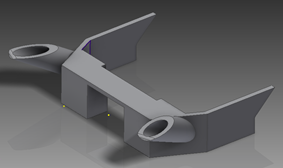
\includegraphics[width=0.28\textwidth]{figs/CADHeck.png}}
		\hspace{0.5cm}
		\subfigure[Pi-Ständer und Powerpackhalterung]		{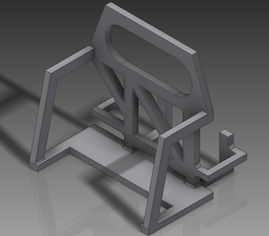
\includegraphics[width=0.28\textwidth]{figs/CADPiStaender.png}}
		\hspace{0.5cm}
		\subfigure[Teile verbaut im Roboter]		{\includegraphics[width=0.28\textwidth]{figs/CADEingebaut.png}}
		\caption{Gehäuseteile des Roboter aus dem 3D-Drucker}
		\label{fig:Gehäuseteile}
	\end{figure}
\end{center}
Für die CAD-Zeichnungen wurden die Studentenversion von Autodesk Inventor Professional 2014 verwendet. Bild a) zeigt das Heckteil, das lediglich für die Optik entworfen wurde, wohingegen das Teil aus Bild b9, der Pi-Ständer, mehrere  praktische Funktion hatte, wie in Bild c) deutlich wird. Durch das aufstellen des Pis wurde Platz auf dem Oberdeck des Chassis gespart, sodass das Powerpack dort mit einer Halterung verstaut werden konnte. Das Bauteil Pi-Ständer hält außerdem das Powerpack in Position und das Langloch im oberen Bereich dient als Griff zum Anfassen und sorgenfreiem Aufnehmen des Roboters. Da beim Anfassen des Roboters anfänglich immer darauf geachtet werden musste, wo man ihn am besten anfässt, um keine Kabel zu lösen oder ähnliches, konnte der Roboter nun bedenkenlos hochgehoben werden.  


\subsection{Sensorik}

Zur Bewältigung einzelner Meilensteine wurden im Laufe der Veranstaltung Programmierung mechatronischer Systeme verschiedene Sensoren implementiert. Diese wurden über ein Breadboard mit Steckverbindungen an den Raspberry Pi angeschlossen. 

\subsubsection{Liniensensor}

Für den ersten Meilenstein (siehe Kapitel 3.1) standen Sensoren des Typs \glqq \textit{Grove Line Finder v1.0}\grqq \ der Firma \glqq \textit{Seedstudio Groove}\grqq \ bereit. Bei diesen handelt es sich um Infrarot-Sensoren, die IR-Licht über eine Infrarot-Leucht-Diode auf den Boden strahlen. Das reflektierte Licht wird über einen Fototransistor ausgewertet. Über die Intensität der Reflketion sind sie in der Lage zwischen weißem und schwarzen Untergrund zu unterscheiden. Über ein Potentiometer auf dem Sensor ist es möglich die Sensitivität des Sensors und somit einen Schwellwert des Schaltens der Transistoren anzupassen. Bei schwarzem Untergrund schaltet der Transistor und der Sensor gibt einen \glqq \textit{High-Pegel}\grqq \ aus. Die Spannung dieses Ausgangs entspricht der Versorgungsspannung des Sensors, welche 5 Volt beträgt und direkt vom Raspberry-Pi abgegriffen werden kann. Da die GPIO-Pins des Pi eine maximale Eingangsspannung von 3,3 Volt zulassen, wird das 5 Volt Signal des Sensors über eine Schutzschaltung auf den Raspberry-Pi gegeben. Das Ausgangssignal des Sensors wird dabei über einen Widerstand von $1 k\Omega$ auf die Basis eines NPN-Transistors des Typs \glqq \ 2N3904\grqq \ gegeben (QUELLE). Am Kollektor liegen 3,3 Volt des Raspberry-Pi an und werden beim Schalten des Transistors direkt auf einen GPIO des Raspberry-Pi zurückgeführt (siehe Abbildung \ref{fig:transistor}). Über 3D-gedruckte Komponenten werden die Sensoren an der Plattform montiert, um einen möglichst geringen Abstand zum Boden zu gewährleisten. Dies ist notwendig, um Störeinflüsse des Lichts so weit wie möglich zu umgehen. Um dies noch weiter zu unterstützen, wurde im Rahmen dieser Arbeit beide Liniensensoren mit Abschirmvorrichtungen in Form von dunklen Papiertrichtern versehen, um das Infrarotlicht stärker auf einen Bereich des Untergrunds zu fokussieren und weiter vor Störeinflüssen zu schützen. 

\begin{figure}[!htb]
	\centering
	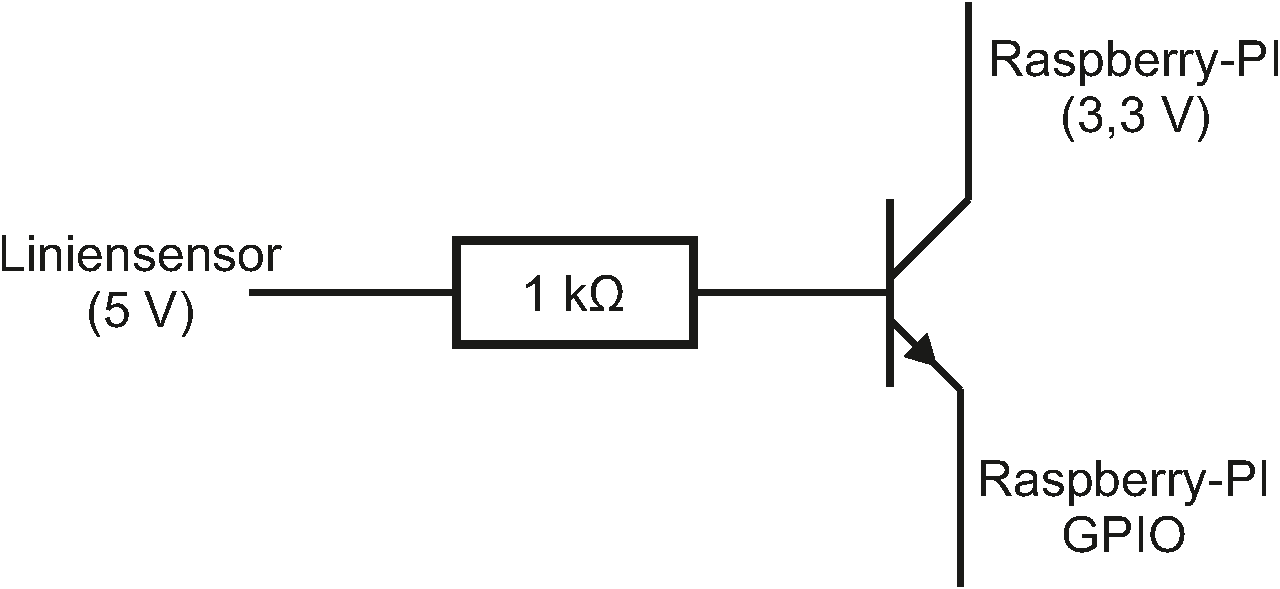
\includegraphics[scale=.3]{figs/transistor}
	\caption{Schaltung der Transistor-Schutzschaltung des Liniensensors}
	\label{fig:transistor}
\end{figure}

\subsubsection{Encoder}

Zur Erfassung der Motorgeschwindigkeiten wurden Encoder oder auch Drehgeber verwendet. Diese bestehen aus zwei Hallsensoren und einer rotierenden Magnetscheibe mit 6 Polpaaren (siehe Abbildung \ref{fig:encoder}). Nach dem Prinzip eines stromdurchflossenen Leiters in einem Magnetfeld ergibt sich beim Durchlauf des Hallsensors eine Spannung die proportional zum Produkt aus magnetischer Feldstärke und Stromstärke des Leiters ist. Die sich bei einer rotierenden Magnetscheibe einstellenden Spannungssprünge, werden als Encoder-Ticks bezeichnet und sind Grundlage zur Drehzahlberechnung. Bei einer vollständigen Umdrehung der Magnetscheibe ergeben sich bei zwei Hallsensoren somit 12 verwendbare Impulse. Der Spannungspegel entspricht dabei der Versorgungsspannung der Hallsensoren von 3,3 Volt, welche direkt vom Raspberry-Pi gespeist wird.\\ 
Da der Encoder nicht direkt an die Motorwelle angeschlossen ist, sondern sich auf der Abtriebsseite eines Getriebes mit einer Getriebeübersetzung von 120:1 befindet, vervielfältigt sich diese Anzahl zu 1440 Impulsen bei einer Radumdrehung. Die Auflösung ist somit ausreichend hoch für eine genaue und schnell abgetastete Drehzahlerfassung, die für regelungstechnische Zwecke eingesetzt werden kann. Während der Fahrt werden die Impulse des Encoders kontinuierlich über einen separaten Thread ausgelesen, um ein Fehler während schnellen Impulsmessung zu vermeiden.

\begin{figure}[!htb]
	\centering
	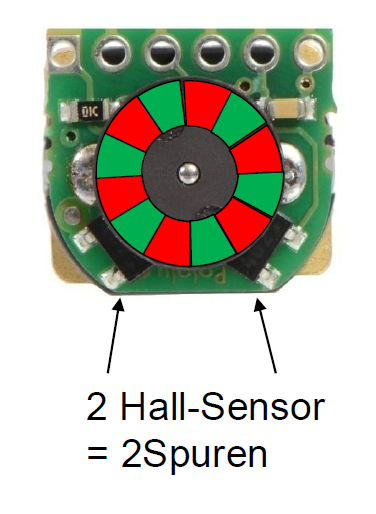
\includegraphics[scale=.3]{figs/encoder}
	\caption{Aufbau des verwendeten Drehgebers basierend auf dem Hall-Effekt QUELLE!}
	\label{fig:encoder}
\end{figure}

\subsubsection{Ultraschallsensoren}

Zur Distanzmessung wurden im Rahmen des dritten Meilensteins (Vergleiche Kapitel 3.3) und der \glqq \textit{Roboter-Challange}\grqq \ Ultraschallsensoren vom Typ \glqq \textit{Grove Ultrasonic Finder}\grqq \  der Firma \glqq \textit{Seedstudio Groove}\grqq \  bereitgestellt. Sie dienen der berührungslosen Abstandsmessung und können bei einer Auflösung von $1 cm$ einen Bereich von $3 - 400 cm$ messen (QUELLE!). Bei der Abstandsmessung wird ein Ultraschallsignal mit einer Frequenz von $40 kHz$ ausgesandt. Dabei wird die Zeit $\Delta t$ gemessen, die das Echo an der Wand benötigt, um wieder zum Sensor zurückzukehren. Mit der gemessenen Zeit und der konstanten Schallgeschwindigkeit unter thermodynamischen Grundbedingungen von $v_{sonic} = 343.2$ ergibt sich eine Abstand $d$ nach Gleichung \ref{eq:ultrasonic}. Dabei wird durch zwei geteilt, da die halbe Distanz berechnet werden soll, die der Schall zurücklegt.

\begin{center}
	\begin{equation}
	d =  v_{sonic} \cdot \frac{\Delta t}{2}
	\label{eq:ultrasonic}
	\end{equation}
\end{center} 

Um die Abstandsmessung zu starten muss ein \glqq \textit{High-Pegel}\grqq \ über $10 \mu s$ auf einen Pin des Sensors gegeben werden. Nach 8 internen $40 kHz$-Impulsen des Ultraschallsensors wird dann auf eine Antwort des Sensors in Form eines \glqq \textit{High-Pegels}\grqq \ gewartet. Die gemessene Zeit des Pegels entspricht dann der in Gleichung \ref{eq:ultrasonic} verwendeten Zeit $\Delta t$ über die sich der Abstand berechnen lässt. Das Senden und Empfangen der Daten läuft dabei über den selben Pin des Sensors. Im Programmcode ist es dementsprechend beim Ansprechen des Sensors notwendig den GPIO des Raspberry-Pi öfters zwischen Eingang und Ausgang umzukonfiguriren. Da der Sensor mit einer Spannung von 5 Volt versorgt wird, und diese auch als Pegel ausgibt, ist aus dem gleichen Grund wie beim Liniensensor eine Schutzschaltung zu implementieren. Da diese jedoch sowohl Eingangs- als auch Ausgangssignale verarbeiten können muss, wird eine Spannungsteiler- anstelle einer Transistorschutzschaltung verwendet. Für weitere Informationen sei an dieser Stelle auf QUELLE! verwiesen.

\subsubsection{Farbsensor}

\newpage
%-----------------------------
% Softwaretechnische Umsetzung
%-----------------------------
\section{Umsetzung der Meilensteine}

	
\subsection{Linie folgen}
\textit{}	

Im Rahmen des ersten Meilensteins, gilt es einer weißen Linie auf schwarzem Untergrund zu folgen. Der Linienverlauf beinhaltet dabei sowohl Geradeausverläufe, als auch Links- und Rechtsabbiegungen in Form von S-Kurven und 90-Grad-Abbiegungen. Zwei der in Kapitel 2.2 beschriebenen digitalen Infrarot-Spursensoren werden zur Ermittlung der Position des Roboters entlang der besagten Linie montiert und angeschlossen. Die Schnittstelle zum Auslesen der digitalen Signale der Sensoren liefert eine Klasse \textit{Liniensensor}, welche eine Methode zur Erfassung digitaler Pegel bereitstellt. Sie liest einen Anschlusspin des RaspberryPi aus und detektiert, ob sich der Roboter über weißem oder schwarzem Untergrund befindet. Für jeden Sensor wird ein Objekt des Typs \textit{Liniensensor} in der Klasse \textit{Mobileplatform} erstellt.

Zur Linienfahrt ergeben sich drei Ansätze, die auf der Orientierung besagter Spursensoren basieren: Das Verfolgen einer Linienkante, Platzierung beider Sensoren auf der Linie und Positionierung rechts und links neben der Linie. Im Rahmen dieser Arbeit wurde der letzte Ansatz gewählt, da er sich bei der Implementierung als robuster erwiesen hat und sich zugleich ein ruhigeres Fahrverhalten einstellte.

Basierend auf der zuvor genannten Lösungsstrategie, ergibt sich die Implementierung des Algorithmus. Ein Programmablaufplan dessen ist in Abbildung ... zu sehen. Er hat die Aufgabe die Sensoren während der Fahrt stets links und rechts neben der weißen Linie zu halten. Der Aufruf des Algorithmus erfolgt in der Klasse \textit{Mobileplatform} über eine ungetaktete While-Schleife, sodass kontinuierlich der Status beider Sensoren abgefragt wird. Detektieren die Liniensensoren beide schwarzen Untergrund, befinden sich die Sensoren in ihrer Soll-Position und der Roboter fährt geradeaus. Ist gibt der linke Sensor einen \textit{Low-Pegel} zurück, befindet sich dieser über weißem Untergrund. Der Roboter ist zu weit nach rechts abgewichen. Es folgt eine Korrektor der Ausrichtung anhand einer Linksdrehung. Analog Erfolgt bei einem \textit{Low-Pegel} des rechten Sensors eine Rechtsdrehung.

\begin{figure}[!htb]
	\centering
	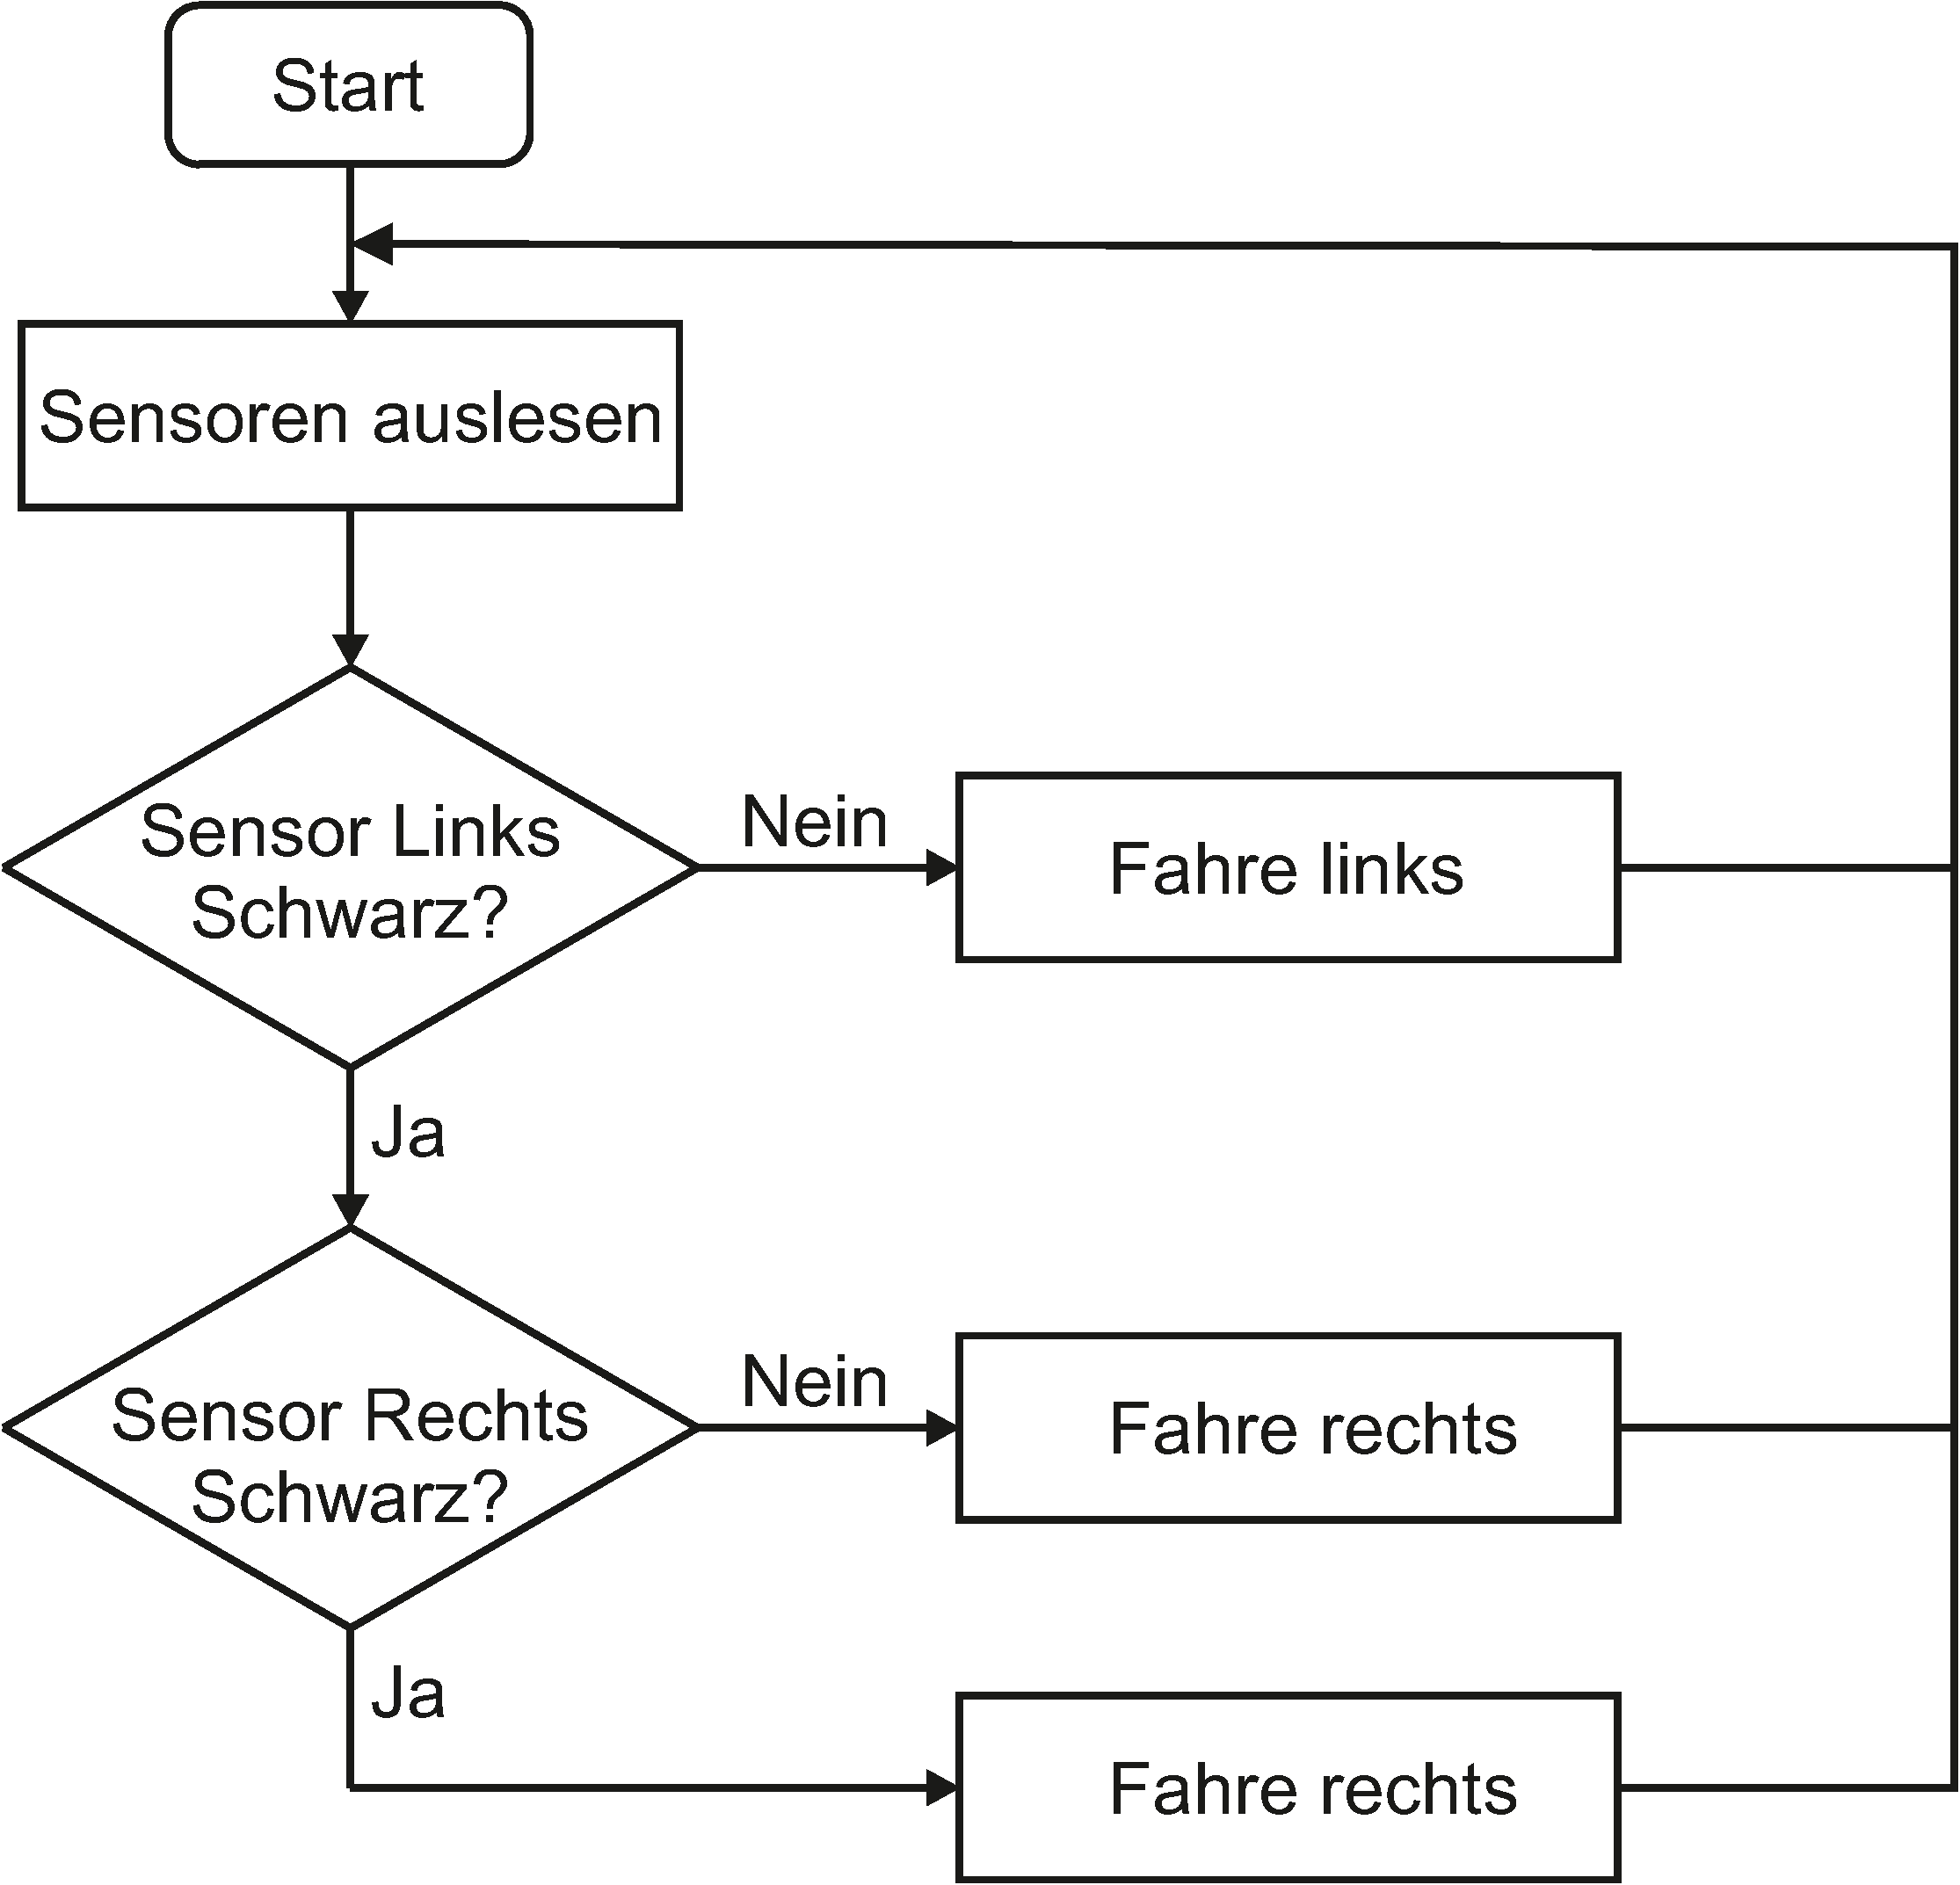
\includegraphics[scale=.3]{figs/PAP_Linie.pdf}
	\caption{Programmablaufplan der Linienfahrt}
	\label{fig:PAP_Linie}
\end{figure}


Die Bewältigung der Aufgabe lief mit dem gewählten Lösungsansatz problemlos. Dies ist unter anderem aber auch auf die stets nahezu konstante Breite der weißen Linie zurückzuführen. Sobald der Abstand der Sensoren geringer ist, als die besagte Breite, versagt die gewählte Lösungsstrategie. Unter dieser Bedingung ist erfahrungsgemäß der Ansatz zur Orientierung an Linienkanten zu wählen. \\
Zudem hatten hohe Geschwindigkeiten aufgrund der Massenträgheit zur Folge, dass der Roboter besonders bei 90-Grad-Abbiegungen nicht rechtzeitig abbremst und die Linie verlässt. Durch die Detektion schwarzen Untergrunds beider Sensoren, betrachtet der Algorithmus den Roboter in seiner Soll-Position und lässt ihn geradeaus fahren. Um diesem Versagen des Algorithmus entgegenzuwirken, wurde die Fahrtgeschwindigkeit angepasst.
%Abbildungen: PAP, Schematisch Lösungsstrategien, Linienverläufe

	
\subsection{Kreisfahrt}

Die Kreisfahrt war Bestandteil des zweiten Meilensteins. Unter Vorgabe eines Radius im Bereich von 15-35 Zentimeter, galt es den Roboter einen Kreis fahren zu lassen. Dieser durfte einen Toleranzbereich von $\pm$ 2cm nicht verlassen. Zur Überprüfung wurde ein Stift am Roboter befestigt, welcher auf einer Kreisschablone die gefahrene Strecke des Roboters aufzeichnet. Zwei der in Kapitel 2.2 beschriebenen Encoder wurden angeschlossen und eine Klasse \textit{Encoder} in \textit{Dcmotor} integriert(Siehe Abbildung ...). Des weiteren wurde eine Regelung der Geschwindigkeit in der Klasse \textit{Dcmotor} implementiert. Der Algorithmus zur Kreisfahrt wurde schließlich in eine Funktion geschrieben, die die Berechnung der Geschwindigkeiten beider Gleichstrommotoren realisiert. 

Über zwei Hall-Sensoren und ein Getriebe mit einer Übersetzung von 120:1 \cite{Dem13} ergeben sich pro Radumdrehung 1440 Signalflanken des Drehgebers. Über einen Zeitraum von $\Delta T = 0.1s$ werden Impulse $k$ gezählt und nach Gleichung \ref{eq:calcSpeed} unter Berücksichtigung des Raddurchmessers von $d = 0,063m$ zu einer Geschwindigkeit in SI-Basiseinheiten umgerechnet.

\begin{center}
\begin{equation}
v = \frac{k d \pi}{1440\Delta T}
\label{eq:calcSpeed}
\end{equation}
\end{center} 

Da der Signalpegel des Drehgebers im Zeitraum von 0,1 Sekunden ausreichend hoch ist, um eine Geschwindigkeit zu berechnen, kann Messrauschen durch ungenaue Fertigung der Encoder vernachlässigt werden. Demzufolge führt die Mittelwertbildung mehrerer Drehzahlsignale zu keiner Verbesserung in der Regelung.

Zur Regelung wird ein PID-Regler mit einer Taktrate von $10Hz$ implementiert. Somit wird bei jeder Erfassung der aktuellen Geschwindigkeit eine Änderung dieser durch den Regler vorgenommen. Abbildung \ref{fig:PID_controller}  zeigt ein Blockschaltbild des verwendeten PID-Reglers. 

\begin{figure}[!htb]
	\centering
	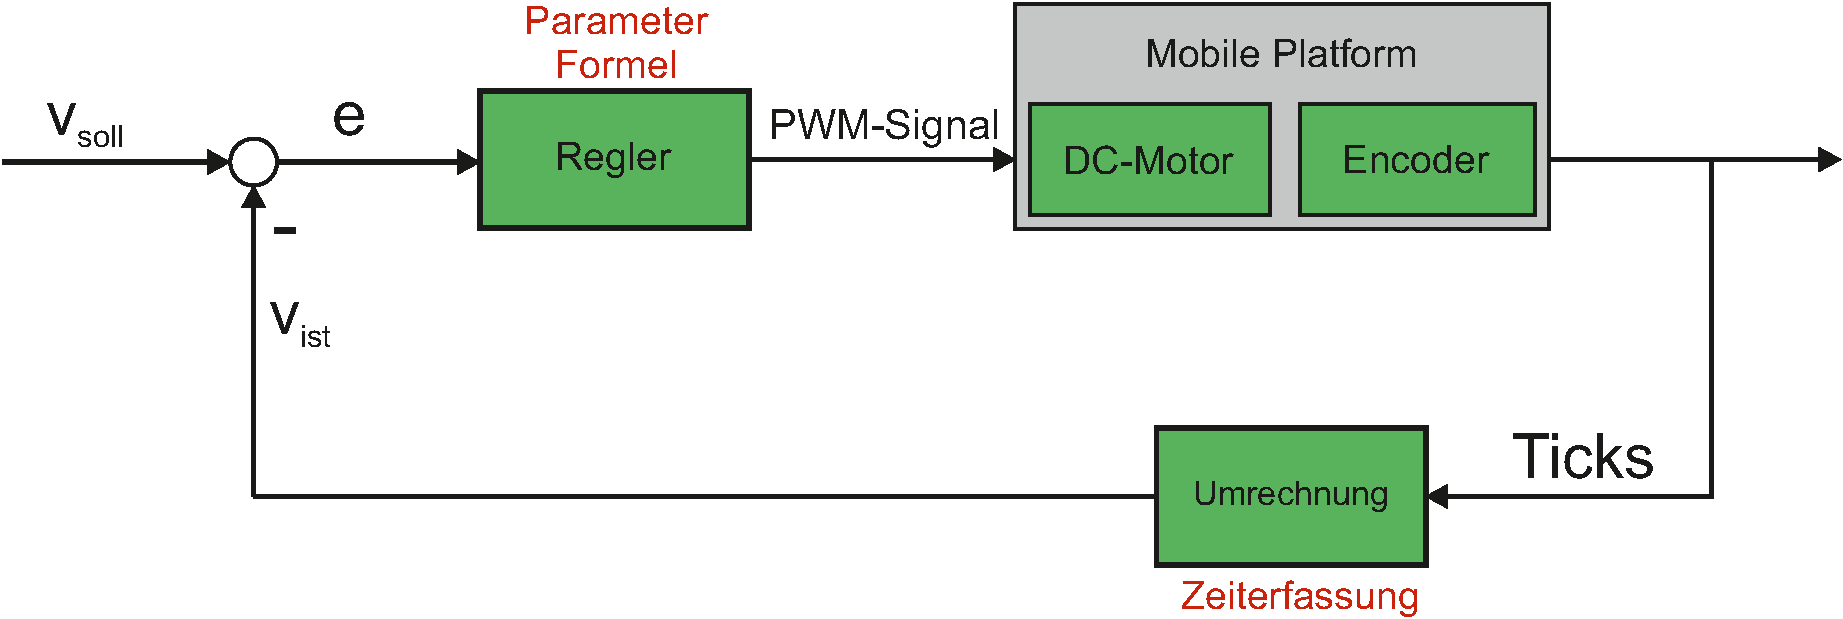
\includegraphics[scale=.5]{figs/PID_controller}
	\caption{Blockschaltbild eines PID-Reglers}
	\label{fig:PID_controller}
\end{figure}

Die Eingangsgröße des Reglers ergibt sich aus der Differenz und somit dem Fehler $e$ aus Ist-Geschwindigkeit $v_{ist}$ und Soll-Geschwindigkeit$v_{soll}$. Diese Differenz wird nach Formel \ref{eq:pidController} durch einen proportionalen , integralen und differentiellen Anteil so verstärkt, dass sich die Regelabweichung verkleinert und im optimalen Fall verschwindet. Der proportionale Anteil verstärkt dabei den Fehler mit einem konstanten Faktor $K_{P}$. Da der es sich um einen zeit diskreten Regler handelt, bildet sich der integrale Anteil nicht durch eine Integration der Regelabweichung über die Zeit, sondern. durch die Multiplikation der Summe aller Fehler mit der Konstanten $K_{I}$. Analog dazu wird der differenzielle Anteil nicht nach der Zeit abgeleitet sondern ergibt sich aus dem Produkt der Differenz des Fehlers mit dem Fehler des vergangenen Abtastschrittes und dem Faktor $K_{D}$. 

\begin{center}
	\begin{equation}
	y[n] =  K_{P}\cdot e[n] + K_{I} \cdot \sum\limits_{m=0}^n e[m] \cdot \Delta T+ K_{D} \cdot \frac{e[n] - e[n-1]}{\Delta T}
	\label{eq:pidController}
	\end{equation}
\end{center} 

Die Verstärkungen der Regler werden über $Live-Tuning$, das heißt im laufenden Betrieb des Roboters ermittelt. Eine Auslegung der Parameter über ein lineares Systemmodell zweiter Ordnung ist nur schwer möglich, da das Übertragungsverhalten von Geschwindigkeit und PWM-Signal nichtlinear ist. Dieses Verhalten ist in der Kennlinie von Abbildung \ref{fig:nl_kennlinie_R} zu entnehmen.
Des Weiteren wurden für beide Motoren verschiedene Parameter ermittelt, da sie bei gleichem Eingangssignal unterschiedliche Drehzahlen aufweisen. 

\begin{figure}[!htb]
	\centering
	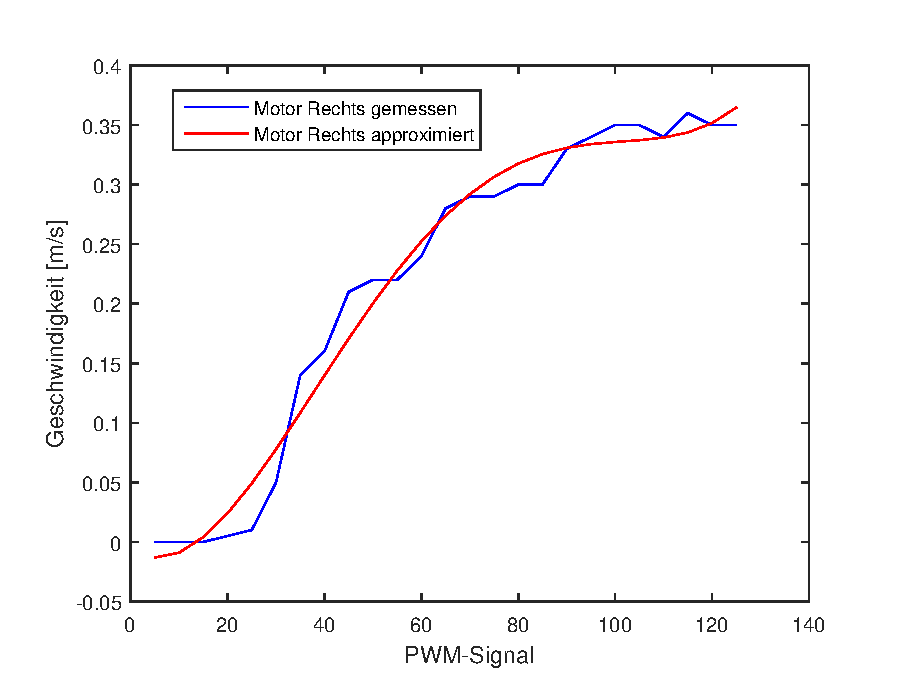
\includegraphics[scale=.7]{figs/Motor_Rechts_Kennlinie.eps}
	\caption{Nichtlineare Kennlinie der Drehzahl des rechten Motors}
	\label{fig:nl_kennlinie_R}
\end{figure}

\newpage
Zur Realisierung der Kreisfahrt im Uhrzeigersinn wurde die Klasse \textit{Mobileplatform} um eine Methode erweitert, die eine Funktion zur Berechnung der einzelnen Radgeschwindigkeiten bereitstellt. Die Basisgeschwindigkeit wird dabei zwischen beiden Rädern angenommen (Abbildung \ref{fig:kreisfahrt}), deren Abstand ($b=11cm$) beträgt. Da die Distanz von Mittelpunkt zu Stifthalter ($s = 12 cm$), welcher am hinteren Ende des Roboters befestigt wurde, nicht vernachlässigbar ist, fließt dessen Position in die Berechnung der Geschwindigkeiten mit ein. Aus Abbildung \ref{fig:kreisfahrt}, die eine Rotation des Roboters um einen Punkt P darstellt, folgen die Gleichungen \ref{eq:kreisfahrt1}, \ref{eq:kreisfahrt2} und \ref{eq:kreisfahrt3} zur Berechnung der Soll-Geschwindigkeiten.

\begin{center}
	\begin{equation}
		r_{soll} = \sqrt{r^2-s^2}
	\label{eq:kreisfahrt1}
	\end{equation}
\end{center} 

\begin{center}
	\begin{equation}
	v_{Links} = v \cdot \frac{r + \frac{b}{2}}{r}
	\label{eq:kreisfahrt2}
	\end{equation}
\end{center} 

\begin{center}
	\begin{equation}
	v_{Rechts} = v \cdot \frac{r - \frac{b}{2}}{r}
	\label{eq:kreisfahrt3}
	\end{equation}
\end{center}


\begin{figure}[!htb]
	\centering
	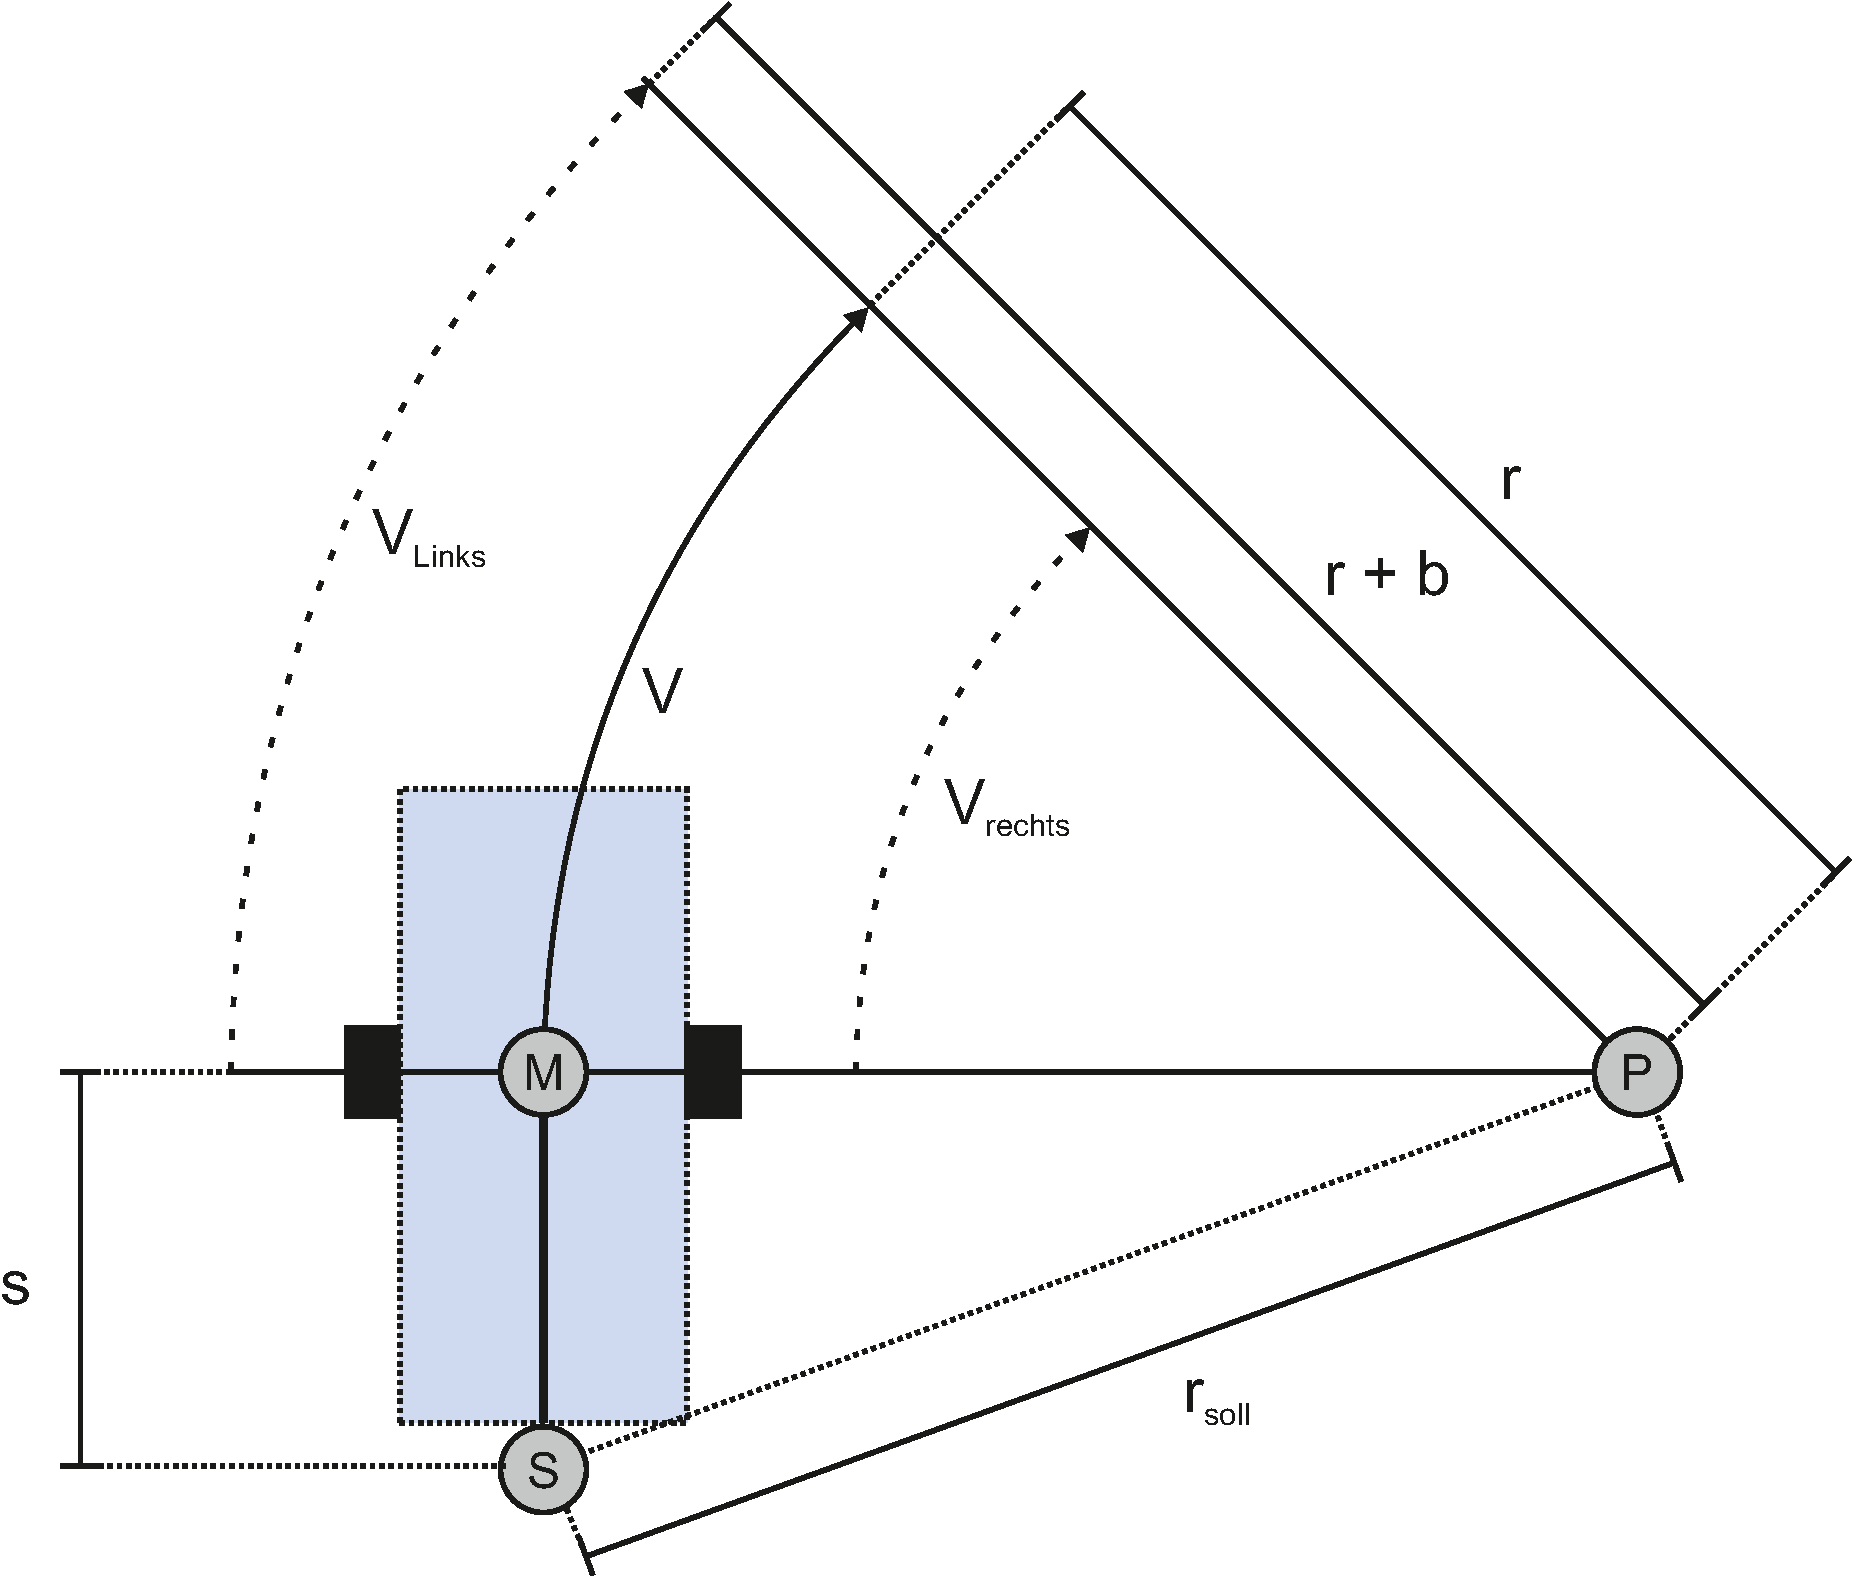
\includegraphics[scale=.4]{figs/Kreisfahrt}
	\caption{Nichtlineare Kennlinie der Drehzahl des rechten Motors}
	\label{fig:kreisfahrt}
\end{figure}


\newpage
Bei der Abnahme des Meilensteins wurden Radien von 23 und 30 cm abgefahren. Dies lief bei $r_{soll} = 23 cm$ problemlos. Nur beim Radius von 30 cm gab es kleine Überschreitungen der Toleranzgrenze von $\pm$ 2cm. Da die Signale der Encoder ausreichend hochauflösend sind, ist dieser Fehler hauptsächlich auf die Einschwingvorgänge des Reglers und Messunsicherheiten der Geometrien zurückzuführen. 

In den weiteren Aufgabenteilen wird die Geschwindigkeitsregelung beibehalten, da sie die Laufruhe des Roboters unterstützt und auch dabei hilft Hindernisse zu überwinden.




	
\subsection{Kollisionsfreie Korridorfahrt}

Herausforderung des 3. Meilensteins war eine autonome, kollinsionsfreie Fahrt durch ein Labyrinth mit einem konstanten Wandabstand von 35 cm. Die Rechts- und Linksabbiegungen der Strecke verlaufen dabei alle mit einem Winkel von 90 Grad. Als kollisionfrei wurde im Kontext der Vorlesung als grundsätzlich kontaktfrei von Objekten in der Umgebung definiert, also war auch keine streifen von Objekten zulässig. Die Berührung der zur Auswahl gestellten Tastsensoren mit den Wänden wurde jedoch nicht als Kollision gewertet. Da mit den Ultraschallsensoren eine quasi kontinuierliche Abstandsmessung möglich war und
mit den Tastern nur ein definierter Abstand detektiert werden konnte, fiel die Wahl auf die
Ultraschallsensoren zur Navigation der Plattform. Zur Messung des absoluten Abstands von Roboter zu Wand wurden somit zwei der besagten Sensoren (siehe Kapitel 2.2) angeschlossen und über einer Klasse \textit{Ultrasonic} angesprochen. Die Sensoren werden nacheinander ausgelesen um Interferenzen und somit Fehler bei der Distanzmessung zu vermeiden. Des weiteren wurden die Ultraschallsensoren nicht direkt seitlich an der Plattform angebracht, sondern mit einem leichten Winkelversatz von $\alpha = 30^{\circ}$ nach vorne montiert. Abbildung \ref{fig:kurve} zeigt, dass dies ein Vorausschauen des Roboters und somit die rechtzeitige Erkennung von Abbiegungen bewirkt. 

\begin{figure}[!htb]
	\centering
	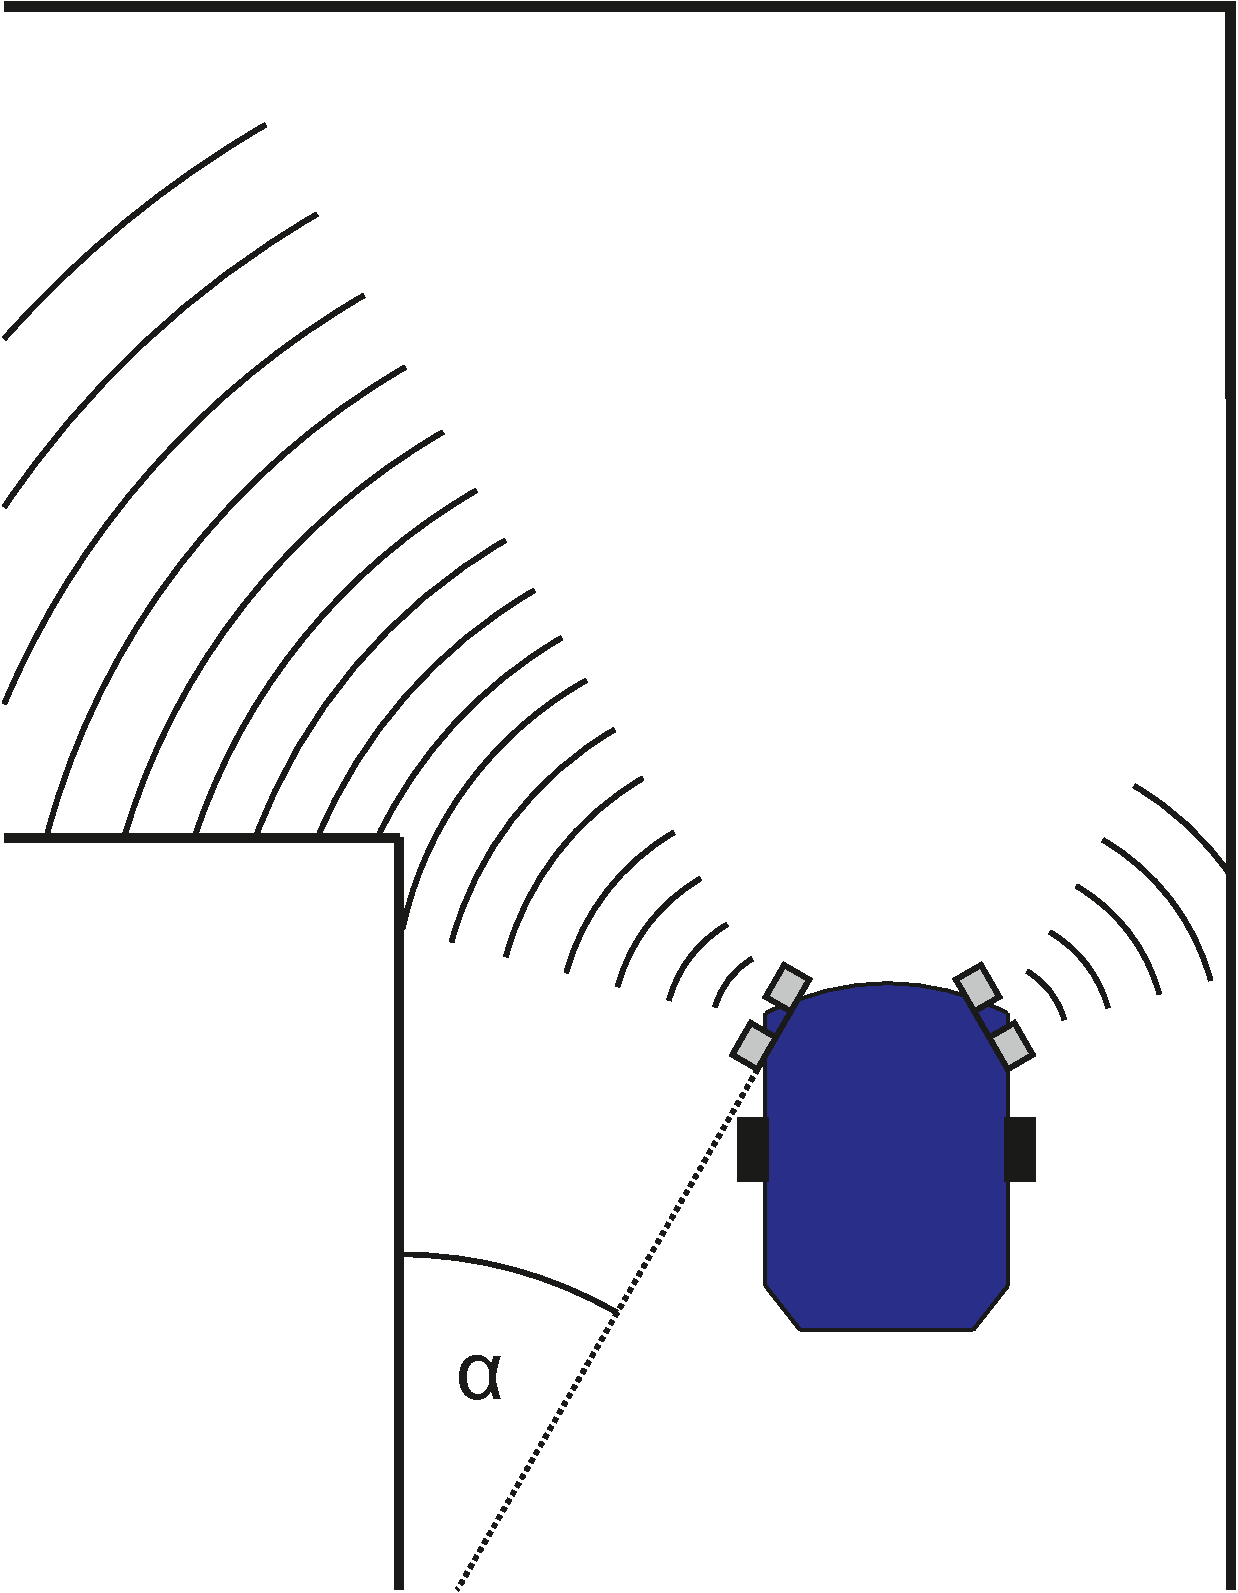
\includegraphics[scale=.3]{figs/kurve}
	\caption{Anbringung der Ultraschallsensoren im Hinblick auf Kurvenverhalten}
	\label{fig:kurve}
\end{figure}

Das UML-Diagramm in Abbildung ... veranschaulicht, den Zusammenhang der Klasse \textit{Mobileplatform} und \textit{Ultrasonic}. Es ist ersichtlich, dass \textit{Mobileplatform} vollständigen zugriff auf Funktionalitäten der Ultraschallsensoren erhält. Somit eignet sich diese Klasse gut für die Implementierung des Algorithmus zur Korridorfahrt, der die Erkennung von Hindernissen gewährleisten soll. Zur Regelung des Roboters während der Fahrt wurden im Rahmen dieser Arbeit drei verschiedene Ansätze mir unterschiedlicher Anordnung der Ultraschallsensoren erprobt. Diese verschiedenen Strategien werden im Folgenden erläutert und durch Abbildung \ref{fig:ansatz} unterstützt.

\begin{figure}[!htb]
	\centering
		\subfigure[Berücksichtung Winkelversatz]
		{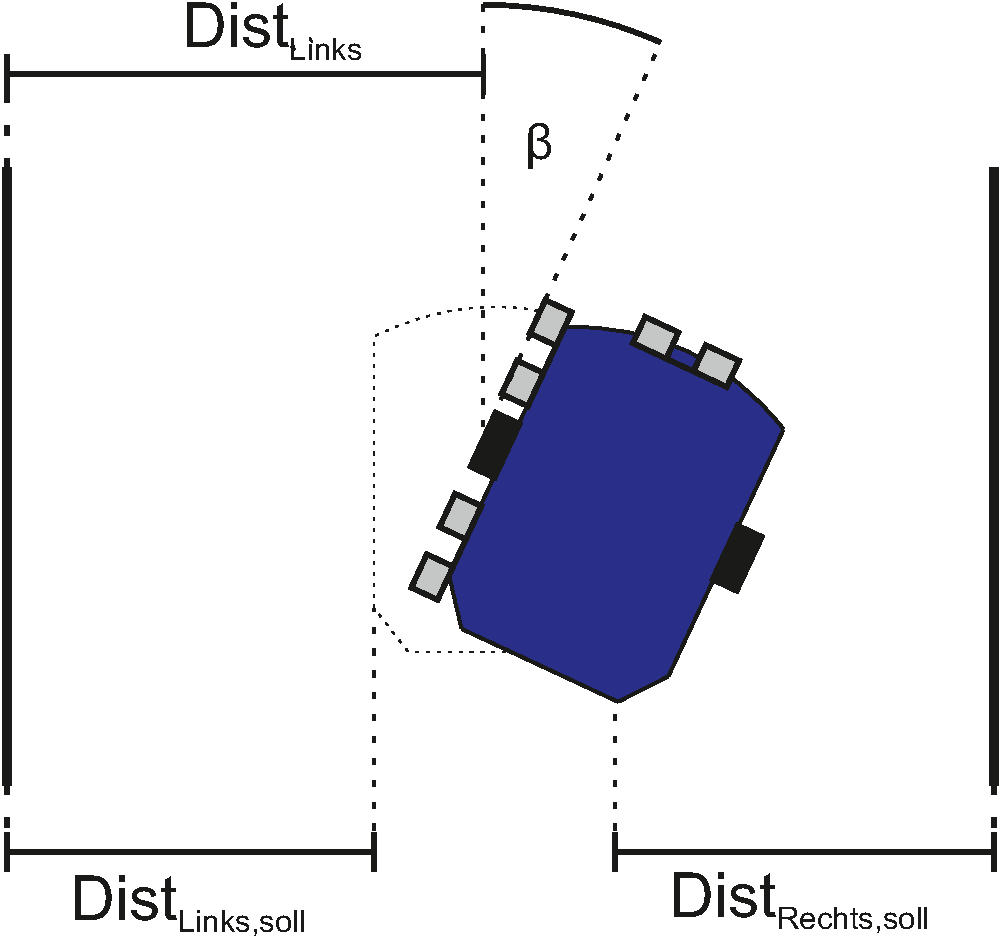
\includegraphics[scale=.35]{figs/ansatz2}}
	\hspace{5mm}
	\subfigure[Distanzmessung beider Seiten]
	{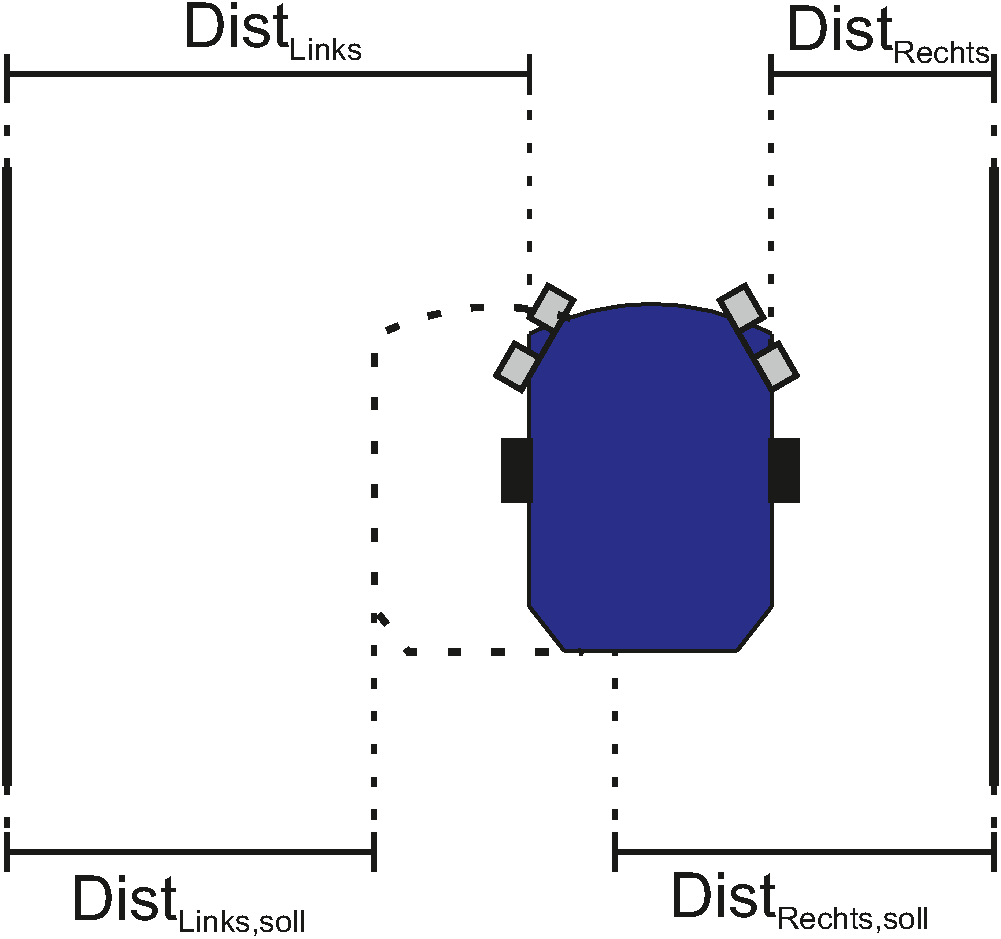
\includegraphics[scale=.35]{figs/ansatz}}
	\caption{Position des Roboters im Korridor}
	\label{fig:ansatz}
\end{figure}

In Abbildung \ref{fig:ansatz}(a) sind zwei Sensoren seitlich am Roboter montiert und einer in Fahrtrichtung. Der Ansatz des Algorithmus beruht auf einer Orientierung an der Linken Wand des Korridors. Dabei werden wird sowohl der Winkelversatz der seitlich montierten Sensoren, als auch der Abstand zur linken Wand während Fahrt des Roboters berücksichtigt und gegebenenfalls korrigiert. Der vordere Sensor detektiert, ob sich ein Hindernis in Fahrtrichtung befindet und ein Abbiegevorgang ausgeführt werden muss. Aufgrund von Schwierigkeiten der Implementierung eines Kaskadereglers mit Winkel- Abstandskorrektur wurde dieser Ansatz aufgrund von Zeitmangel verworfen. Zudem hätte ein Abbiegevorgang implementiert werden müssen, was als \glqq Hard Coding\grqq \ gilt und im Vergleich zum Regleransatz unelegant und nicht wiederverwendbar ist.\\
Der zweite und dritte erprobte Ansatz wurde mit der zuvor beschriebenen winkelversetzten Sensorkonfiguration ausgeführt. Beide Ansätze beruhen darauf eine Soll-Distanz zu beiden Wänden einzuhalten und den Roboter somit mittig im Korridor zu halten (Abbildung \ref{fig:ansatz}). \\
Dies wurde im Rahmen des zweiten Ansatzes dadurch realisiert, das Verhältnis aus $Dist_{Links}$ und $Dist_{Rechts}$ mit der Initialgeschwindigkeit des jeweiligen Motors zu multiplizieren. Somit ergeben sich nach Gleichung \ref{eq:verhaeltnis1} und \ref{eq:verhaeltnis2} für beide Räder neue Soll-Geschwindigkeiten. Diese Geschwindigkeiten sind dabei auf einen Bereich zwischen $0,05$ und $0.4$ Meter pro Sekunde begrenzt.

\begin{center}
	\begin{equation}
	v_{Rechts} = v \cdot \frac{Dist_{Links}}{Dist_{Rechts}}
	\label{eq:verhaeltnis1}
	\end{equation}
\end{center}

\begin{center}
	\begin{equation}
	v_{Links} = v \cdot \frac{Dist_{Rechts}}{Dist_{Links}}
	\label{eq:verhaeltnis2}
	\end{equation}
\end{center} 

Da sich bei Abbiegungen ein entsprechend großes Verhältnis einstellt, ist dieser Ansatz auch für Abbiegevorgänge geeignet. \\
Als dritte Option, wurde eine Abstandsregelung mittels zweier P-Regler implementiert. Diese setzte sich im aufgrund ihrer Robustheit und sich einstellenden Fahrtruhe gegen die zuvor genannten Verfahren durch. Da die Ultraschallsensoren, aufgrund ihrer Positionierung nicht den direkten Abstand zur Wand messen, wurde zur Bestimmung der Soll-Größen eine Referenzmessung durchgeführt, bei der der Roboter mittig im Korridor platziert wurde. Somit ergab sich bei mittiger Fahrt eine minimale Regelabweichung $e$. Ein Blockdiagramm des verwendeten P-Reglers ist in Abbildung \ref{fig:pcontrol} zu sehen.\\

\begin{figure}[!htb]
	\centering
	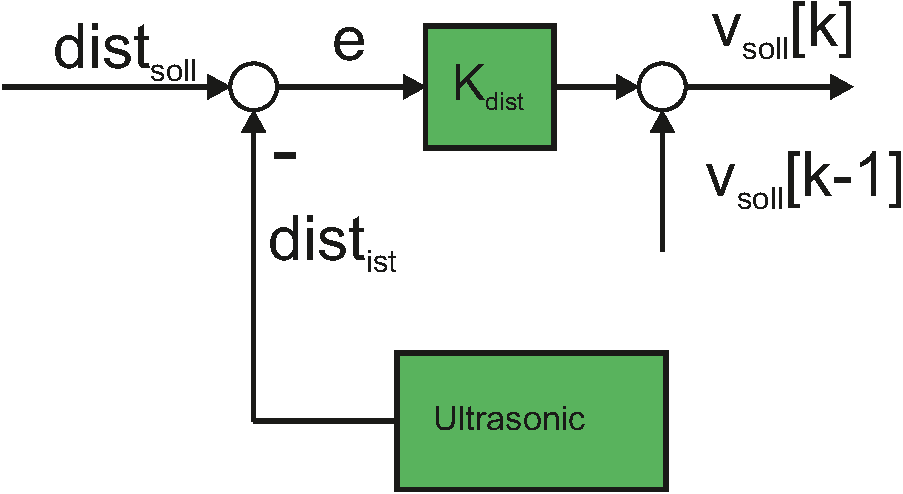
\includegraphics[scale=.5]{figs/Pcontrol}
	\caption{Anbringung der Ultraschallsensoren im Hinblick auf Kurvenverhalten}
	\label{fig:pcontrol}
\end{figure}

Die Ermittlung der proportionalen Regelverstärkung erfolgte empirisch. Dabei musste ein Kompromiss aus steiler Kurveneinlenkung und ruhiger Geradeausfahrt gefunden werden. Abbildung ... zeigt, dass sich bei geringen Verstärkungen der Regeldifferenz zwar ein ruhiges Fahrverhalten auf gerader Strecke ergibt, das Einlenken in Kurven jedoch durch zu träge ist und zu Kollisionen führen kann. Analog dazu ergibt sich bei großer Fehlerverstärkung eine ungleichmäßige, zur Seite schwingende Geradeausfahrt, die bis zum Kontakt mit den Seitenwänden führen dann. In Kurven agiert der Roboter hingegen hoch dynamisch (Abbildung \ref{fig:pcontrolgain}). 

\begin{figure}[!htb]
	\centering
	\subfigure[Große Verstärkung]
	{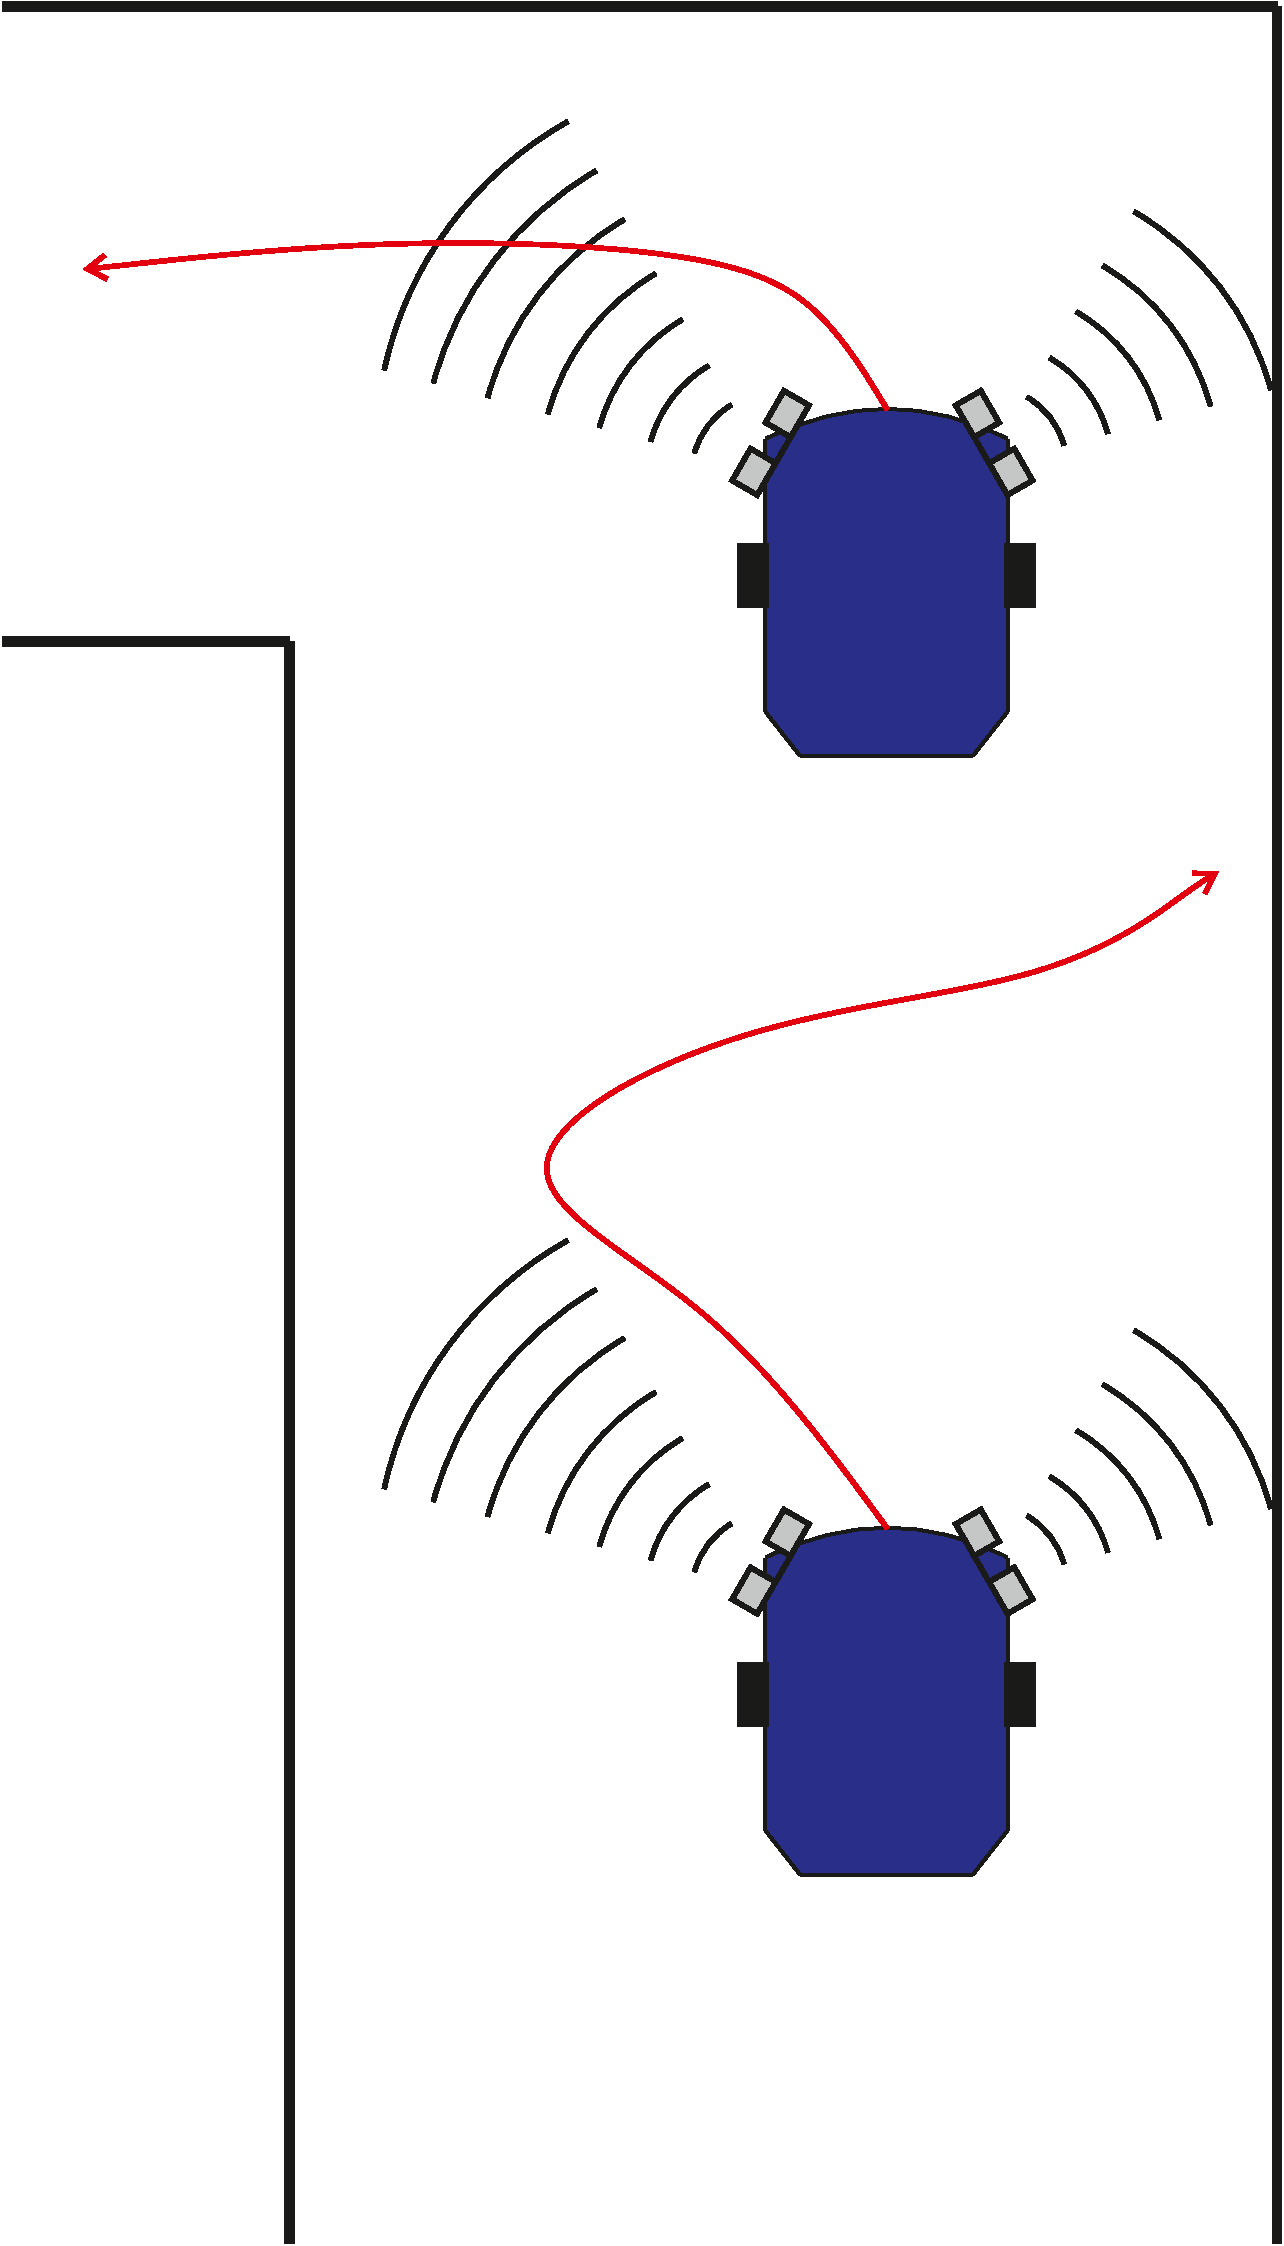
\includegraphics[scale=.25]{figs/highgain}}
	\hspace{5mm}
	\subfigure[Geringe Verstärkung]
	{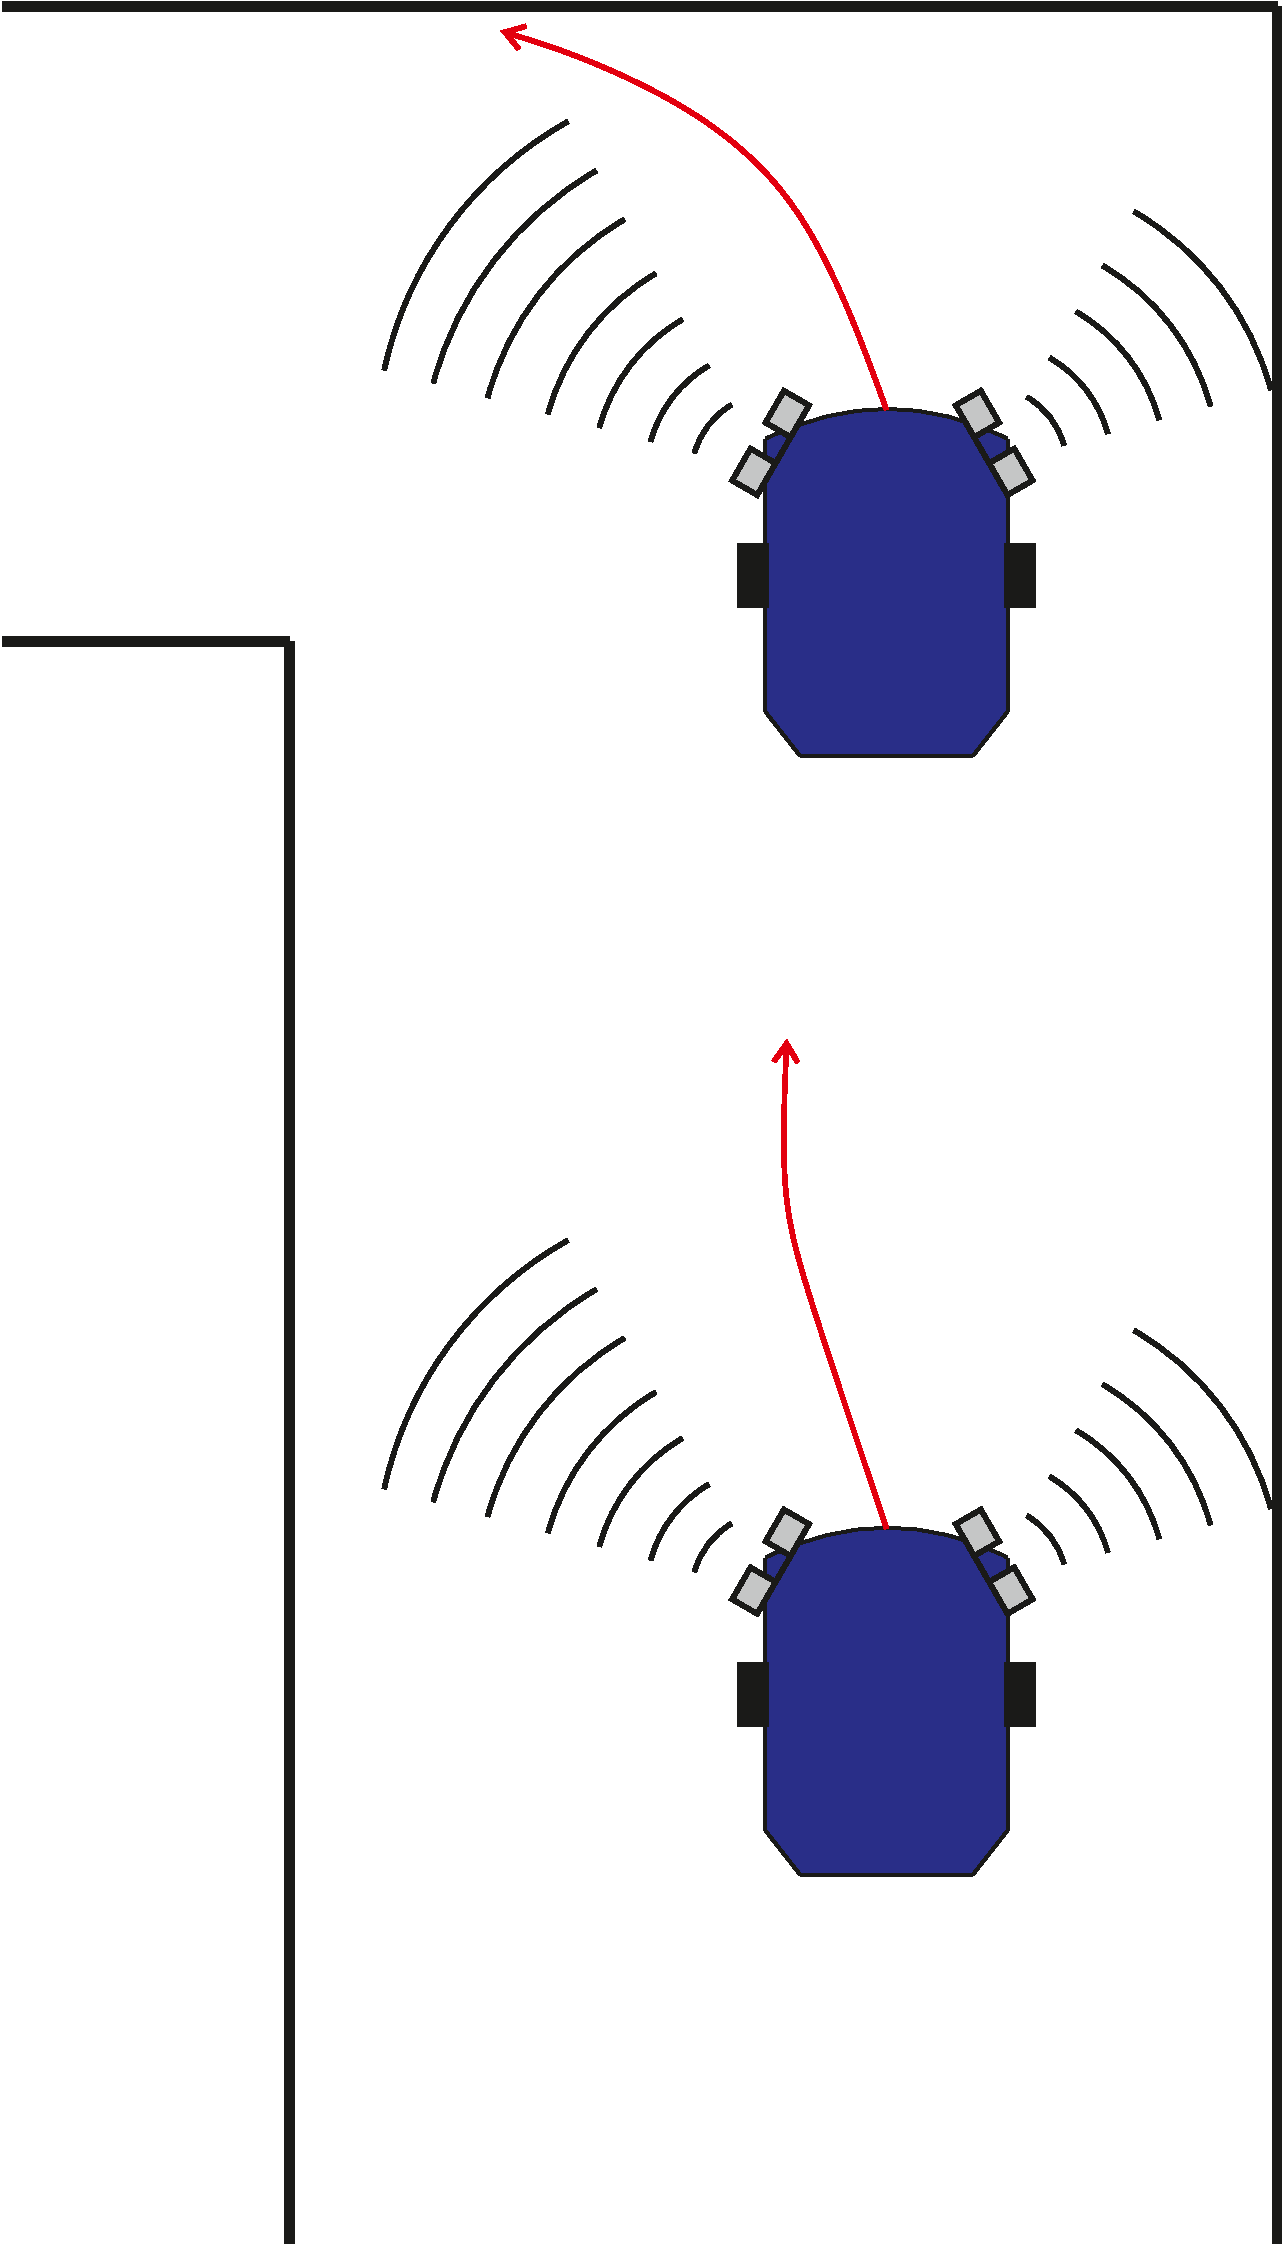
\includegraphics[scale=.25]{figs/lowgain}}
	\caption{Verhalten des proportionalen Verstärkungsfaktors}
	\label{fig:pcontrolgain}
\end{figure}
 \newpage
Ist die Verstärkung zu groß, lenkt der Roboter in einer Linksabbiegung gegebenenfalls zu schnell ein und es ergibt sich eine weitere Situation, die den Algorithmus versagen lässt (Abbildung \ref{fig:UltraschallsensorEckeVerfehlt}). Durch eine große gemessene Distanz des linken Sensors, detektiert der Roboter eine weitere Linksabbiegung und dreht im Labyrinth um oder bleibt im schlechtesten Fall an der Abbiegung stecken.

\begin{center}
	\begin{figure}[!h]
		\centering
		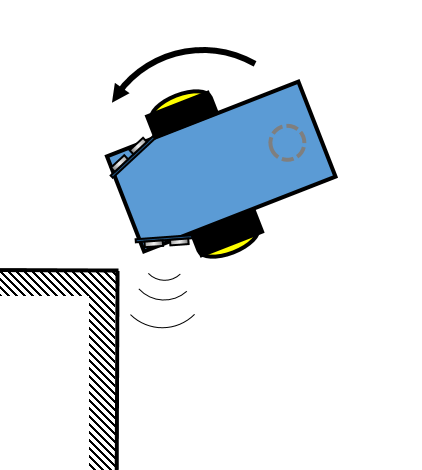
\includegraphics[scale=.4]{figs/EckenProblem.png}
		\caption{Ultraschallsensor detektiert Innenwand nicht mehr}
		\label{fig:UltraschallsensorEckeVerfehlt}
	\end{figure}
\end{center}

\newpage

\subsection{Farbfeld-Suche}
	
Beim letzten Meilensteins, der auch als "Roboter-Challenge" bezeichnet wird, handelt es sich um eine Erweiterung der kollisionsfreien Korridorfahrt. Die abzufahrende Strecke wird vergrößert und um weitere Abbiegungen erweitert, welche nicht mehr nur um 90 Grad, sondern auch in einem beliebigen Winkel abknicken können. Zudem werden im Labyrinth Hindernisse in Form einer Wippe und einer Bodenwelle verteilt und Farbfelder in den Farben Rot, Grün und Blau ausgelegt. Die Hindernisse sind ohne weitere Veränderung des Algorithmus zu bewältigen, was auf den Geschwindigkeitsregler zurückzuführen ist, der einer Verringerung der Geschwindigkeit auf einer Steigung entgegenwirkt. Die Farbfelder der werden über einen RGB-Farbsensor des Typs "FLORA Color Sensor" detektiert. Über eine Klasse \textit{Colorsensor}, die in der \textit{Mobileplatform}  implementiert ist, können die einzelnen RGB-Farben über 16-Bit-Integer ausgelesen werden. Der Parkour ist dann erfolgreich abgeschlossen, wenn der Roboter ohne Kollisionen über die Hindernisse fährt und schließlich auf dem roten Farbfeld stehen bleibt. 
Da für die Parkourfahrt nur das rote Farbfeld von Bedeutung war, wurde die Farbe Rot im
Verhältnis zu Grün und Blau identifiziert. Der Schwellenwerte wurde empirisch ermittelt.\\

Um Störeinflüsse auf die Farbmessung zu filtern, die auf alle drei Farbdioden näherungsweise gleichermaßen wirken, wird der Mittelwert aller Messergebnisse aus einem Messzyklus gebildet (Gl. 6) und anschließend von dem Messwert, den der Sensor lieferte subtrahiert (Gl. 7).
\begin{center}
	\begin{equation}
	average = \frac{redVal_{Sensor}+greenVal_{Sensor}+blueVal_{Sensor}}{3}
	\label{eq:kreisfahrt1}
	\end{equation}
	
	\begin{equation}
	redVal_{filtered} = redVal_{Sensor}-average
	\label{eq:kreisfahrt1}
	\end{equation}
\end{center}

Um das rote Farbfeld robust zu erkennen und nicht mit den weißen Flächen auf der Wippe und dem Bump zu verwechseln, welche ebenfalls den gesamten Rotanteil des Lichts reflektieren, hat sich bei Versuchen herausgestellt, dass es nicht allein reichte einen Bestimmten Grenzwert des gefilterten roten Farbwertes $redVal_{filtered}$ zu betrachten. Es war notwendig den Farbwert des Rotanteils mit dem des Blauanteils in Relation zu setzen. Letzenendes setzte sich folgende Ungleichung mit dem dazugehörigem Schwellwert bei einer robusten Rotfelderkennung durch:

\begin{center}
	\begin{equation}
	220 > redVal_{filtered} - blueVal_{filtered}
	\label{eq:kreisfahrt1}
	\end{equation}
\end{center}

	
	%-----------------------------
	% Diskussion
	%-----------------------------
	\section{Diskussion}
	
	In diesem Abschnitt werden die vier lehrreichsten Hindernisse, die zu überwinden waren, in chronologischer Reihenfolge erörtert. Darauf folgend werden einige Ansätze angesprochen, die bei einer Weiterentwicklung verfolgt worden wären.
	\\
	Der Wunsch unseres Teams besonders gut bei der Vorlesung abzuschneiden und unsere Experimentierfreudigkeit haben dazu geführt, dass stellenweise zu komplexe Lösungsansätze für die Erfüllung der Aufgaben gewählt oder unbewusst Raum für weitere Fehlerquellen geschaffen wurde. Unsere erstes Hindernis bestand aus der Inbetriebnahme der Liniensensoren. Die selbst hergestellte Teststrecke für die Linienfahrt verwendete als Untergrund eine handelsübliche schwarze Pappe, deren einziges Kaufkriterium war, sie müsse eben schwarz sein. Da die Pappe verhältnismäßig stark spiegelte war der Kontrast im infrarotem Lichtspecktrum nicht groß genug um eine robuste schwar-weiß-Unterscheidung gewährleisten zu können. 
	
	Unser nächstes Hindernis war beispielhaft für einen zu komplexen Lösungsansatz: Bei der Reglerauslegung der Motoren für die Kreisfahrt im zweiten Meilenstein haben wir versucht die \textit{Simulink Control Design Toolbox} zur Regelparametrierung zu nutzen. Es wurde eine Methode zur Aufzeichnung einer Identifikationsfahrt der Servomotoren erstellt und anhand dieser Daten das System in Simulink simuliert sowie die Regelparameter bestimmt. Bedauerlicherweise war die Performance nicht ausreichend, da der Roboter nicht gerade aus fuhr und das Fahrverhalten unruhig war. Letzteres lies sich an einem Schwingen der Motorgeäusche erkennen. Nach längerem experimentieren und aus Zeitmangel wurden die Parameter letztenendes heuristisch bestimmt. Hierfür wurden Textboxen im GUI implementiert, um Lifetuning vornehmen zu können. Dies ersparte das vielfache Ändern des Programmcodes, das damit einhergehende neu Kompilieren und ausführen.  
	
	
	Nummer drei und vier der Hindernisse ereigneten sich beim dritten Meilenstein, der Kollisionsfreien Fahrt durch einen Korridor. Aus Beobachtung der Challenge im  Vorjahr und durch Erfahrungswerte von der Linienfahrt im ersten Meilenstein entstand bereits früh der Gedanke einen neuen Ansatz für die Korridorfahrt zu erproben: Da in der Roboter-Challenge die Zeit für das Durchfahren des Korridors wichtig sein würde, sollte sich unser Roboter besonders flüssig durch den Korridor bewegen. Uns fiel auf, dass viele Roboter im Zickzack von Wand zu Wand fuhren. Die Idee war, sich mit zwei seitlich angebrachten Ultraschallsensoren parallel in einem definiertem Abstand zur Wand zu bewegen. Über Triangulation sollte eine Winkel- und Abstandsregelung implementiert werden. 	Dieser Ansatz wurde später verworfen, weil eine stabile Regelung aufgrund der hohen Ungenauigkeiten in der Abstandsmessung nicht gelang. Nicht bedacht wurde, dass zusätzlich zu der Messtolleranz von einem 1 cm (in selbstversuchen bestätigt bei Abständen von 5 - 20 cm) nicht genau festgelegt war von welchem Punkt in der Ferne der Abstand gemessen wurde. So kann ein Objekt auch detektiert werden, wenn die Mittellinie des Ultraschallsensores einige Zentimeter an dem Objekt vorführt.
	Unser viertes Hindernis waren Probleme bei der Abstandsregelung für die Korridorfahrt. Grundsätzlich haben wir versucht die Korridorfahrt   mit softcoding zu lösen, also möglichst wenig vordefinierte Fälle zu programmierung (z.B. eine $45^\circ$ oder $90^\circ$ Drehung), da die Korridorfahrt jedoch eine verhältnissmäßig geringe Komplexität aufwies, wären ein paar mehr Fallunterscheidungen im Quellcode sinnig gewesen, um vorallem die Grundgeschwindigkeit beim Durchfahren des Korridors höher als 15 cm/s anzusetzen. 	
	\vspace{2mm}\\
	In der endgültigen Challenge belegte unser Roboter Rang 4 in der Gesamtwertung. Auffallend war, das die Bestzeit unseres Roboters mit 1 min und 14 sek knapp 30 sek langsamer war als die Zeiten der Erst- und Zweitplatzierten. Unser Roboter bewegte sich flüssig und ohne Zwischenstops durch den Korridor jedoch war die Grundgeschwindigkeit mit 15 cm/s im Schnitt offensichtlich deutlich unter der Durchschnittsgeschwindigkeit der Gewinnerteams. 
	Da das Gewinnerteam die Ultraschallsensoren in der selben Art und Weise an ihrem Roboter befestigt hat, wie wir, sollte für weitere Verbesserungen der Positionsregler besser ausgelegt werden. Desweiteren könnte die Idee eines der anderen Teams aufgenommen werden und eine Vorsteuerung implementiert werden, um die PWM-Drehzahl-Kennlinnie der Motoren zu Linearisieren und somit die Regelung zu verbessern. Außerdem könnte man noch mehr den Kompromiss eingehen und mehr hardcoding für die Korridorfahrt verwenden, um zumindest abschnittsweise schneller fahren zu können. Zum Beispiel das Nutzen von zwei unterschiedlichen pGain-Werten je nach dem ob der Roboter gerade eine Kurvenfahrt durchführt oder eine gerade Passage überwindet. Ein weiterer Ansatz wäre den Error bei der Berechnung der neuen Radgeschwindigkeit quadratisch einfließen zu lassen.    
	%-----------------------------
	% Zusammenfassung
	%-----------------------------
	\section{Zusammenfassung}
	In dieser Hausarbeit wurde ein einfaches mechatronisches System in Form einer manövrierfähigen Roboterplattform mit günstiger Hardware zusammengefügt und programmiert. Beginnend mit der Implementierung einer Fernsteuerung wurde der Programmcode mit Methoden zur Verfolgung einer Linie ergänzt. Als nächstes wurden Encoder angeschlossen, mit deren Einsatz Regler programmiert wurden, die eine Drehzahlsteuerung der Motoren ermöglichten, welche durch das Abfahren eines definierten Kreises bewertet wurden. Im Anschluss daran wurde die Roboterplattform mit Ultraschallsensoren ausgestattet, um autonome Navigationsaufgaben in einer Korridorfahrt meistern zu können. Die Einbindung eines Farbsensors über einen $I^{2}C-Bus$ bildete die letzte Hardwareergänzung für die abschließende Roboter-Challenge. Durch die Wiederverwendbarkeit von Methoden und Klassen wurde eine sukzessive Weiterentwicklung des Programmcodes ermöglicht.
	
	Die Bearbeitung der Teilaufgaben verliefen einzeln sowie im Team zügig und zielorientiert. Detaillierte Absprachen zu den Aufgabenzuweisungen unter den Teammitgliedern ermöglichten die Einhaltung der Meilensteine. Die frühzeitige Bearbeitung der Aufgaben garantierte zum Ende der Fristen hin Kapazitäten um unvorhersehbaren Schwierigkeiten zu meistern. Obwohl der Umfang des endgültigen Programmcodes für routinierte Informatiker überschaubar war, bot er uns zahlreiche Möglichkeiten um die Notwendigkeit eines sauberen und konsequenten Programmierstils zu begreifen und unsere Fähigkeiten im Bereich \textit{Software Engineering} zu vertiefen. Zusätzlich konnten wir theoretische Grundlagen der Reglerauslegung anwenden, elektrische Komponenten Verkabeln und dabei ein praktisches Grundverständnis für Schutzschaltungen und Signalglättung bekommen. 
	
	
	Der Raspberrie Pi 3 lieferte für das Projekt eine zufriedenstellende Performance. Obwohl er über prägnant weniger Rechenleitung verfügt als ein standardmäßiger Personalcomputer verfügt und obwohl der Pi mit bis zu 6 Threads simultan abarbeiten musste, blieb das Fahrverhalten dynamisch und die GUI reagierte in der Regel instantan auf Benutzereingaben.    
	
	\clearpage
	\begin{appendix}
		\section{Abkürzungsverzeichnis}
	\end{appendix}
	\begin{itemize}
		\item PMS - Programmierung mechatronischer Systeme
		\item LKR - Lehrstuhl für Kontinuumsrobotik
		\item C++ - eine Programmiersprache
		\item IDE - Integrierte Entwicklungsumgebung (aus dem Englischen: \textit{integrated development environment})
		\item Qt - das Programm Qt-Creator  
		\item Pi - Raspberry Pi, verwendeter Einplatinencomputer
		\item $I^{2}C$ - Kommunikationsstandard für einen seriellen Datenbus
		\item GPIO - General purpose input output Pins
		\item GUI - Graphical User Interface
		\item PAP - Programmablaufplan nach DIN 66001
		\item SSH - Netzwerkprotokoll (Secure Shell)
		\item RGB - Rot Gelb Blau
		\item PWM - Pulsweitenmodulation 
	\end{itemize} 
	
	
	\clearpage  
	\begin{appendix}
	\section{Programmcode}
	\end{appendix}
    \clearpage  
    %% --- Literaturverzeichnis
    \begin{thebibliography}{50}
   		\bibitem{Dem13} Klaus Dembowski: \textit{Raspberry Pi - Das Handbuch}. Springer Vieweg, ISBN 978-3-658-03166-4, 2013.
	\end{thebibliography}

\end{spacing}
\end{document}                             

